\chapter{Experiments and Results}\label{chapter:experiments_and_results}

This chapter conducts a series of experiments to explore the latent space of the VGG16 model. The first two experiments investigate the small-scale features found in semantically similar images. The subsequent experiments apply the segmentation pipeline introduced in the previous chapter to two well-known datasets. Afterwards, we analyze the feature maps of objects in the foregrounds of multiple images.

\section{Experimental Setup}

In all of our experiments, we used the pretrained VGG16 model from the PyTorch library \parencite{paszke2019pytorch}. We used our own implementation of FSLIC and SFCM but utilized PCA, t-SNE the k-means algorithm available in the Scikit-learn library \parencite{pedregosa2011scikit}. The datasets used were BSD500 \parencite{bsd500} and the Cityscapes dataset \parencite{cityscapes}. BSD500 consists of natural images which have a resolution of $481 \times 321$ while Cityscapes consists of $2048 \times 1024$ images of urban street scenes. BSD500 is a standard dataset for illustrating the capabilities of image segmentation methods. It is semantically similar to the original ImageNet dataset \parencite{deng2009imagenet} on which VGG16 has been trained. Semantic similarity thereby refers to the fact that the images mainly depict a single object or a small number of objects in the foreground and a generic background. Cityscapes, in contrast, contains more complex images with a large number of objects in the foreground and the background.

\section{Exploratory Feature Analysis}

In this section, we discuss two experiments that were conducted to investigate small-scale features among multiple images. The goal of the experiments was to explore the similarities and differences discovered by the model among the images.

\subsection{Visualizing Similar Features}

The first experiment visualized the different features extracted by the VGG16 model in semantically similar images. Due to its high dimensionality, the feature space is difficult to visualize. Therefore, we map vectors in the feature space to the RGB space. The intuition being that similar vectors can be shown together in the form of a pseudo-color image.

% The intuition being that similar feature pixels should be represented by similar RGB colors.

First, a subset of BSD500 containing five semantically similar images was constructed. Next, the 512-dimensional features of the images were extracted from the deepest convolutional layer (block 4) of the network. Then, PCA was applied to obtain a low-dimensional embedding of the feature vectors. Finally, RGB values were extracted from the embeddings by taking the feature projections along the first three principal components and scaling them to lie in the RGB value range. The red, green and blue color channels received their values from the feature projections along the first, second and third principal components, respectively. Since data is maximally varied along the first three principal components, the global dissimilarity between the features can be visualized. It is important to note that PCA was fitted using all of the feature images in the subset. This allowed for a faithful color comparison between the final RGB images. An overview of the process is shown in \autoref{fig:pca_images_process}.

\begin{figure}[t]
    \centering

    
\includegraphics[width=.9\textwidth]{figures/pca_images_process.pdf}
    \caption{An outline of the process to generate RGB feature representative images. The feature images are extracted and their pixels are processed as a batch using PCA. Then, RGB images are constructed from the feature projections along the first, second and third principal components.}
    \label{fig:pca_images_process}
\end{figure}

\autoref{fig:pca_images} shows the results obtained on four subsets of BSD500. As the figure shows, similar objects in the images of every subset are represented with similar colors. This indicates that the VGG16 model has learned to represent (parts of) semantically similar objects with similar hidden representations. Despite the objects of interest having different positions, scales and orientations, the model's object representations are fairly similar. For example, the results in the third subset show similar color distributions in the regions covering the airplanes. Similarly, the regions covering the people shown in the fourth subset have similar colors which indicates that their features lie close to each other in the space of the model. The results obtained from the first two subsets of animals contain a yellow component in the bottom part of the animal and a dark component in the top part of the animal. The top part is usually a weak smooth curve while the bottom part represents the animal's legs.

The color distribution within one image indicates that there is a clear separation between the foreground and the background in the feature image. Due to this separation, clustering the features in a subsequent step can often yield good segmentation masks (as shown in the next section).

\begin{figure}[thbp]
    \centering
    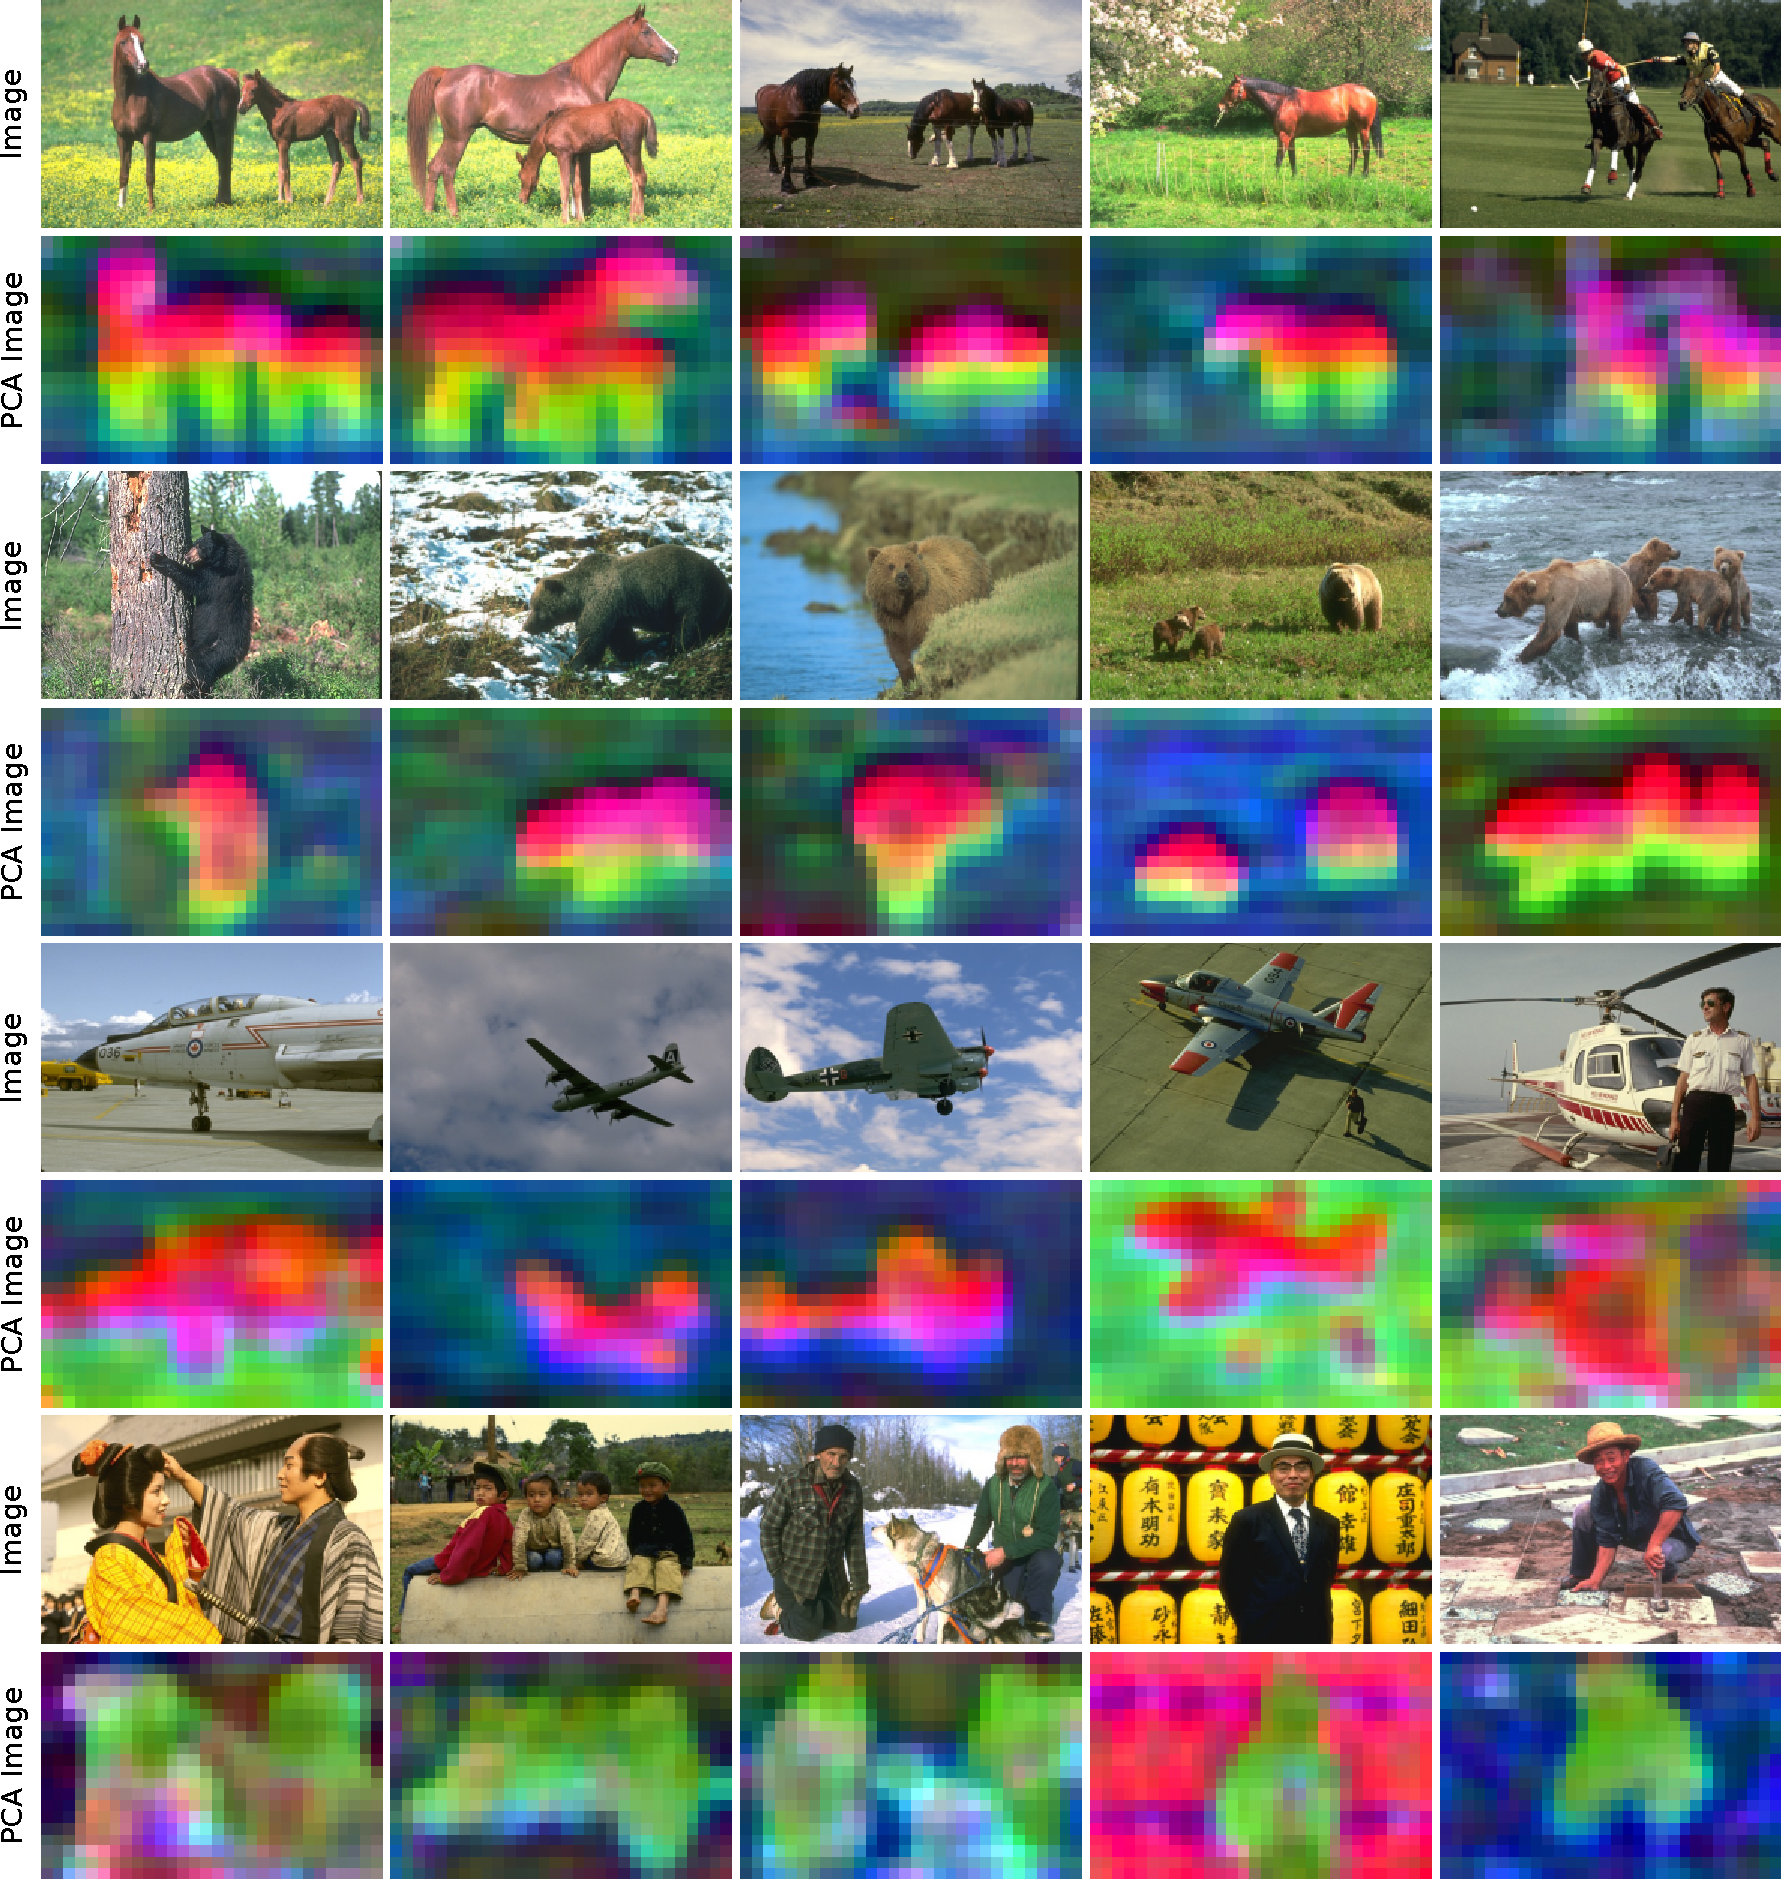
\includegraphics[width=\textwidth]{figures/pca_images.pdf}
    \caption{A figure showing four subsets of BSD500 and their corresponding features mapped to the RGB space. First, a PCA model was fitted using the features of the images in one subset. Then, the features were projected along the first three principal components and their projections were scaled to lie in the RGB value range (PCA Image).}
    \label{fig:pca_images}
\end{figure}

After obtaining the results from BSD500, the same visualization process was applied to images from the Cityscapes dataset. However, since the images contain a greater number of objects, the first three principal components did not capture enough variance in the data and the visualizations obtained were not informative. Therefore, instead of constructing a subset of Cityscapes containing five images, a simpler subset was constructed. The subset consisted of a single image from Cityscapes and two simple images of cars (see \autoref{fig:pca_images_weird}). The idea is that by comparing the colors of the feature mappings from the simple car images with the colors from the Cityscapes scene image, we can verify whether simple objects, such as cars, have a consistent feature representation in more complex images. As shown in \autoref{fig:pca_images_weird}, the cars in all three images are represented by yellow regions, which indicates that they have similar feature representations.

\begin{figure}[t]
    \centering
    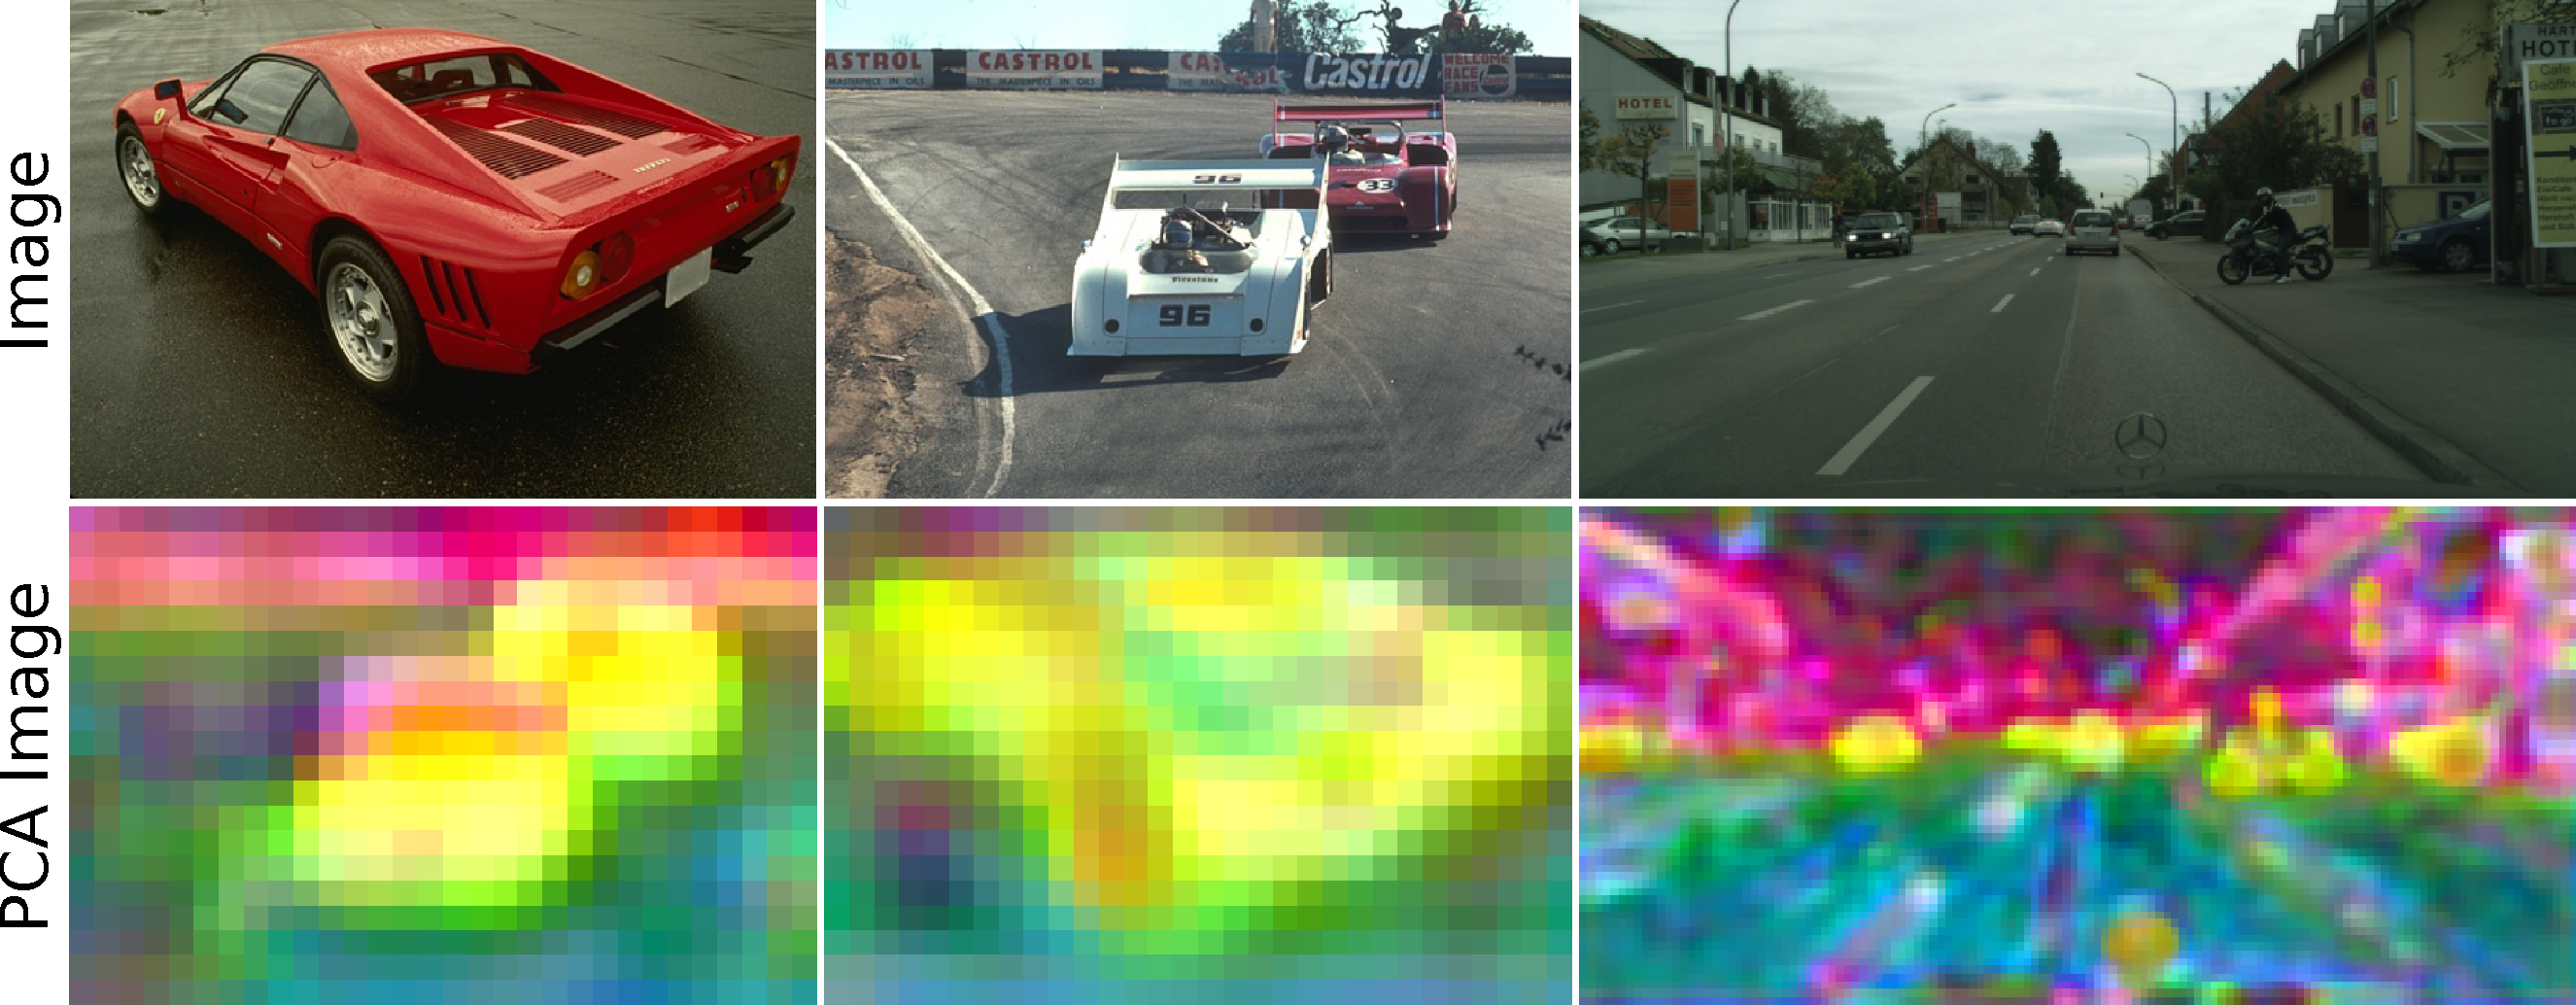
\includegraphics[width=.85\textwidth]{figures/pca_images_weird.pdf}
    \caption{A figure showing three images and their features mapped to RGB space.}
    \label{fig:pca_images_weird}
\end{figure}

We also explored extracting features from the block 3 of VGG16. The intuition is that more general features can be extracted at the early layers. \autoref{fig:pca_images2} shows the results obtained on two subsets of Cityscapes. By looking at the figure, we can see similar general features present in the images of each subset. In both subsets, regions with a large value along the first principal component (indicated by the red areas) appear on object boundaries. In addition, smooth regions have a large value along the third principal component (indicated by the blue areas). These regions include the street and the sidewalk. Finally, areas corresponding to the trees have similar textures and are assigned a large value along the second principal component (indicated by the green areas).

\begin{figure}[htbp]
    \centering
    \includegraphics[width=\textwidth]{figures/pca_images2.pdf}
    \caption{A figure showing two subsets of Cityscapes and their features mapped to RGB space.}
    \label{fig:pca_images2}
\end{figure}

\subsection{Applying t-SNE to Feature Superpixels}

The previous experiment revealed that similar objects were mapped to similar regions in the feature space. Building on that, we conducted a second experiment to create a map of the feature space. The core idea was to extract patches of homogeneous feature representations and to visualize their corresponding ground-truth image patches.

The experiment relied on using t-distributed stochastic neighbor embedding (t-SNE) \parencite{van2008visualizing}. t-SNE is a method which utilizes the local similarity of points lying in high-dimensional space to embed them into a lower dimensional representation (usually 2D or 3D). Points which lie close to each other in the high-dimensional space are modelled using similar lower-dimensional embeddings. t-SNE is typically used for visualization and not for general dimensionality reduction.

The first step of the experiment extracted the feature images of the entire BSD500 from block 4 of the VGG16 model. Then, the feature images were segmented using FSLIC (see \autoref{subsection:color_based_segmentation}) initialized with $K=50$ and $m=0.05$. Afterwards, t-SNE (perplexity=30) was used to embed the centers of the feature superpixels from all the images into a 2D plot. According to t-SNE, similar feature superpixels should lie close to each other in the 2D plot. Finally, each point in the plot was overlayed with a patch representing the part of the original image covered by the superpixel.

\autoref{fig:tsne} shows the results obtained from the experiment. By taking a closer look at the figure, we can see some of the small-scale similarities that the model has found in the dataset. Some of the clusters represent patches with similar patterns such as facial characteristics (\autoref{fig:tsne_clusters} (a)) or areas representing body limbs (\autoref{fig:tsne_clusters} (b)). These patches have similar geometric organizations and color patterns. Other patches represent regions with similar shapes (\autoref{fig:tsne_clusters} (c, e)) or textures (\autoref{fig:tsne_clusters} (d, f)).

\begin{sidewaysfigure}
    \centering
    \includegraphics[width=\textheight]{figures/tsne_plot-compressed.pdf}
    \caption{The result of applying t-SNE (perplexity=30) to feature superpixels extracted from the entire BSD500 dataset. Each patch represents the bounding box of the upsampled feature superpixel superimposed on the original image. The marked regions are shown in \autoref{fig:tsne_clusters}.}
    \label{fig:tsne}
\end{sidewaysfigure}

\begin{figure}[!ht]
    \centering
    \begin{subfigure}[b]{.32\textwidth}
        \centering
        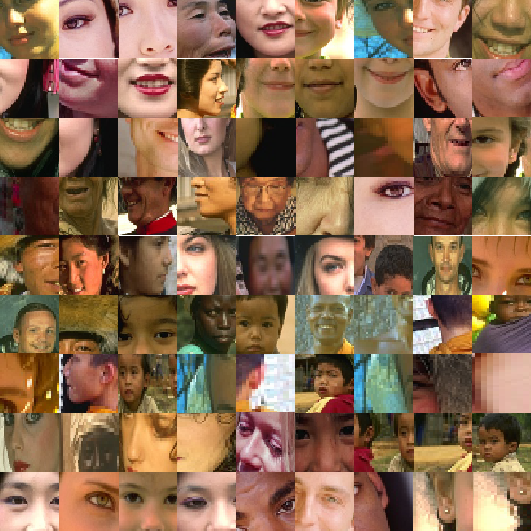
\includegraphics[width=\linewidth]{figures/tsne_a.pdf}
        \caption{}
    \end{subfigure}
    \begin{subfigure}[b]{.32\textwidth}
        \centering
        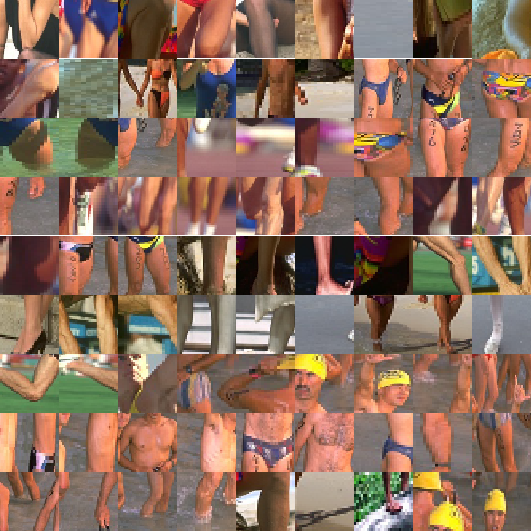
\includegraphics[width=\linewidth]{figures/tsne_b.pdf}
        \caption{}
    \end{subfigure}
    \begin{subfigure}[b]{.32\textwidth}
        \centering
        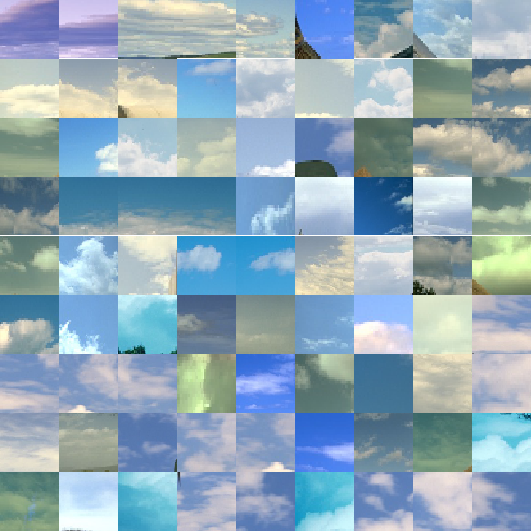
\includegraphics[width=\linewidth]{figures/tsne_c.pdf}
        \caption{}
    \end{subfigure}
    \begin{subfigure}[b]{.32\textwidth}
        \centering
        
\includegraphics[width=\linewidth]{figures/tsne_d.pdf}
        \caption{}
    \end{subfigure}
    \begin{subfigure}[b]{.32\textwidth}
        \centering
        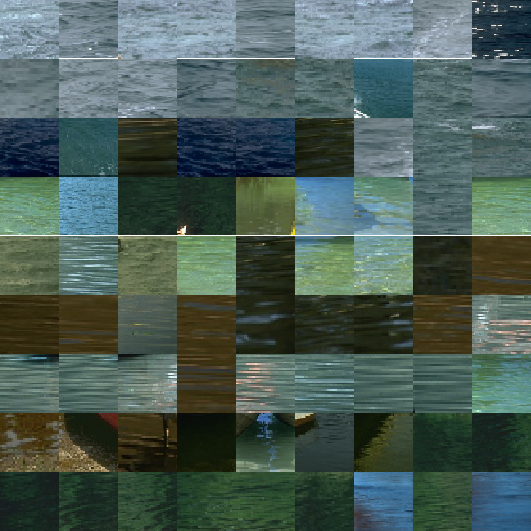
\includegraphics[width=\linewidth]{figures/tsne_e.pdf}
        \caption{}
    \end{subfigure}
    \begin{subfigure}[b]{.32\textwidth}
        \centering
        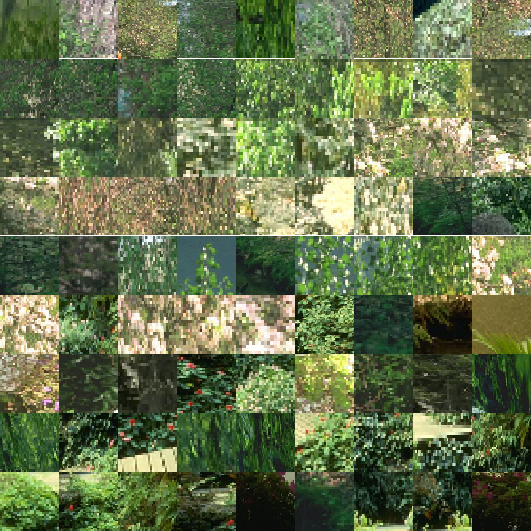
\includegraphics[width=\linewidth]{figures/tsne_f.pdf}
        \caption{}
    \end{subfigure}
    \caption{A figure showing some of the patches found in the regions marked in \autoref{fig:tsne}}
    \label{fig:tsne_clusters}
\end{figure}

\section{Segmentation Experiments}

In this section, we discuss two segmentation experiments conducted on BSD500 and Cityscapes using the pipeline introduced in chapter \ref{chapter:clustering_in_feature_space}. In the first experiment, we extracted object clusters from feature images using the superpixel-based clustering approach. In the second experiment, we extract objects by clustering the pixels of the feature image directly.

\subsection{Clustering Feature Superpixels}

The first experiment extracted the features of six BSD500 images from blocks 2, 3 and 4 of the network. Then, the features were pre-segmented using FSLIC initialized with $m=0.01$. Since the extracted features have different spatial resolutions, the initial superpixel number was set to $K$=1600, $K$=400 and $K$=100 for feature images extracted from block 2, 3 and 4, respectively. Afterwards, the superpixels were clustered using SFCM ($t=1.1$). The silhouette method search interval was set to $[2, 10]$.

\begin{figure}[ht]
    \centering
    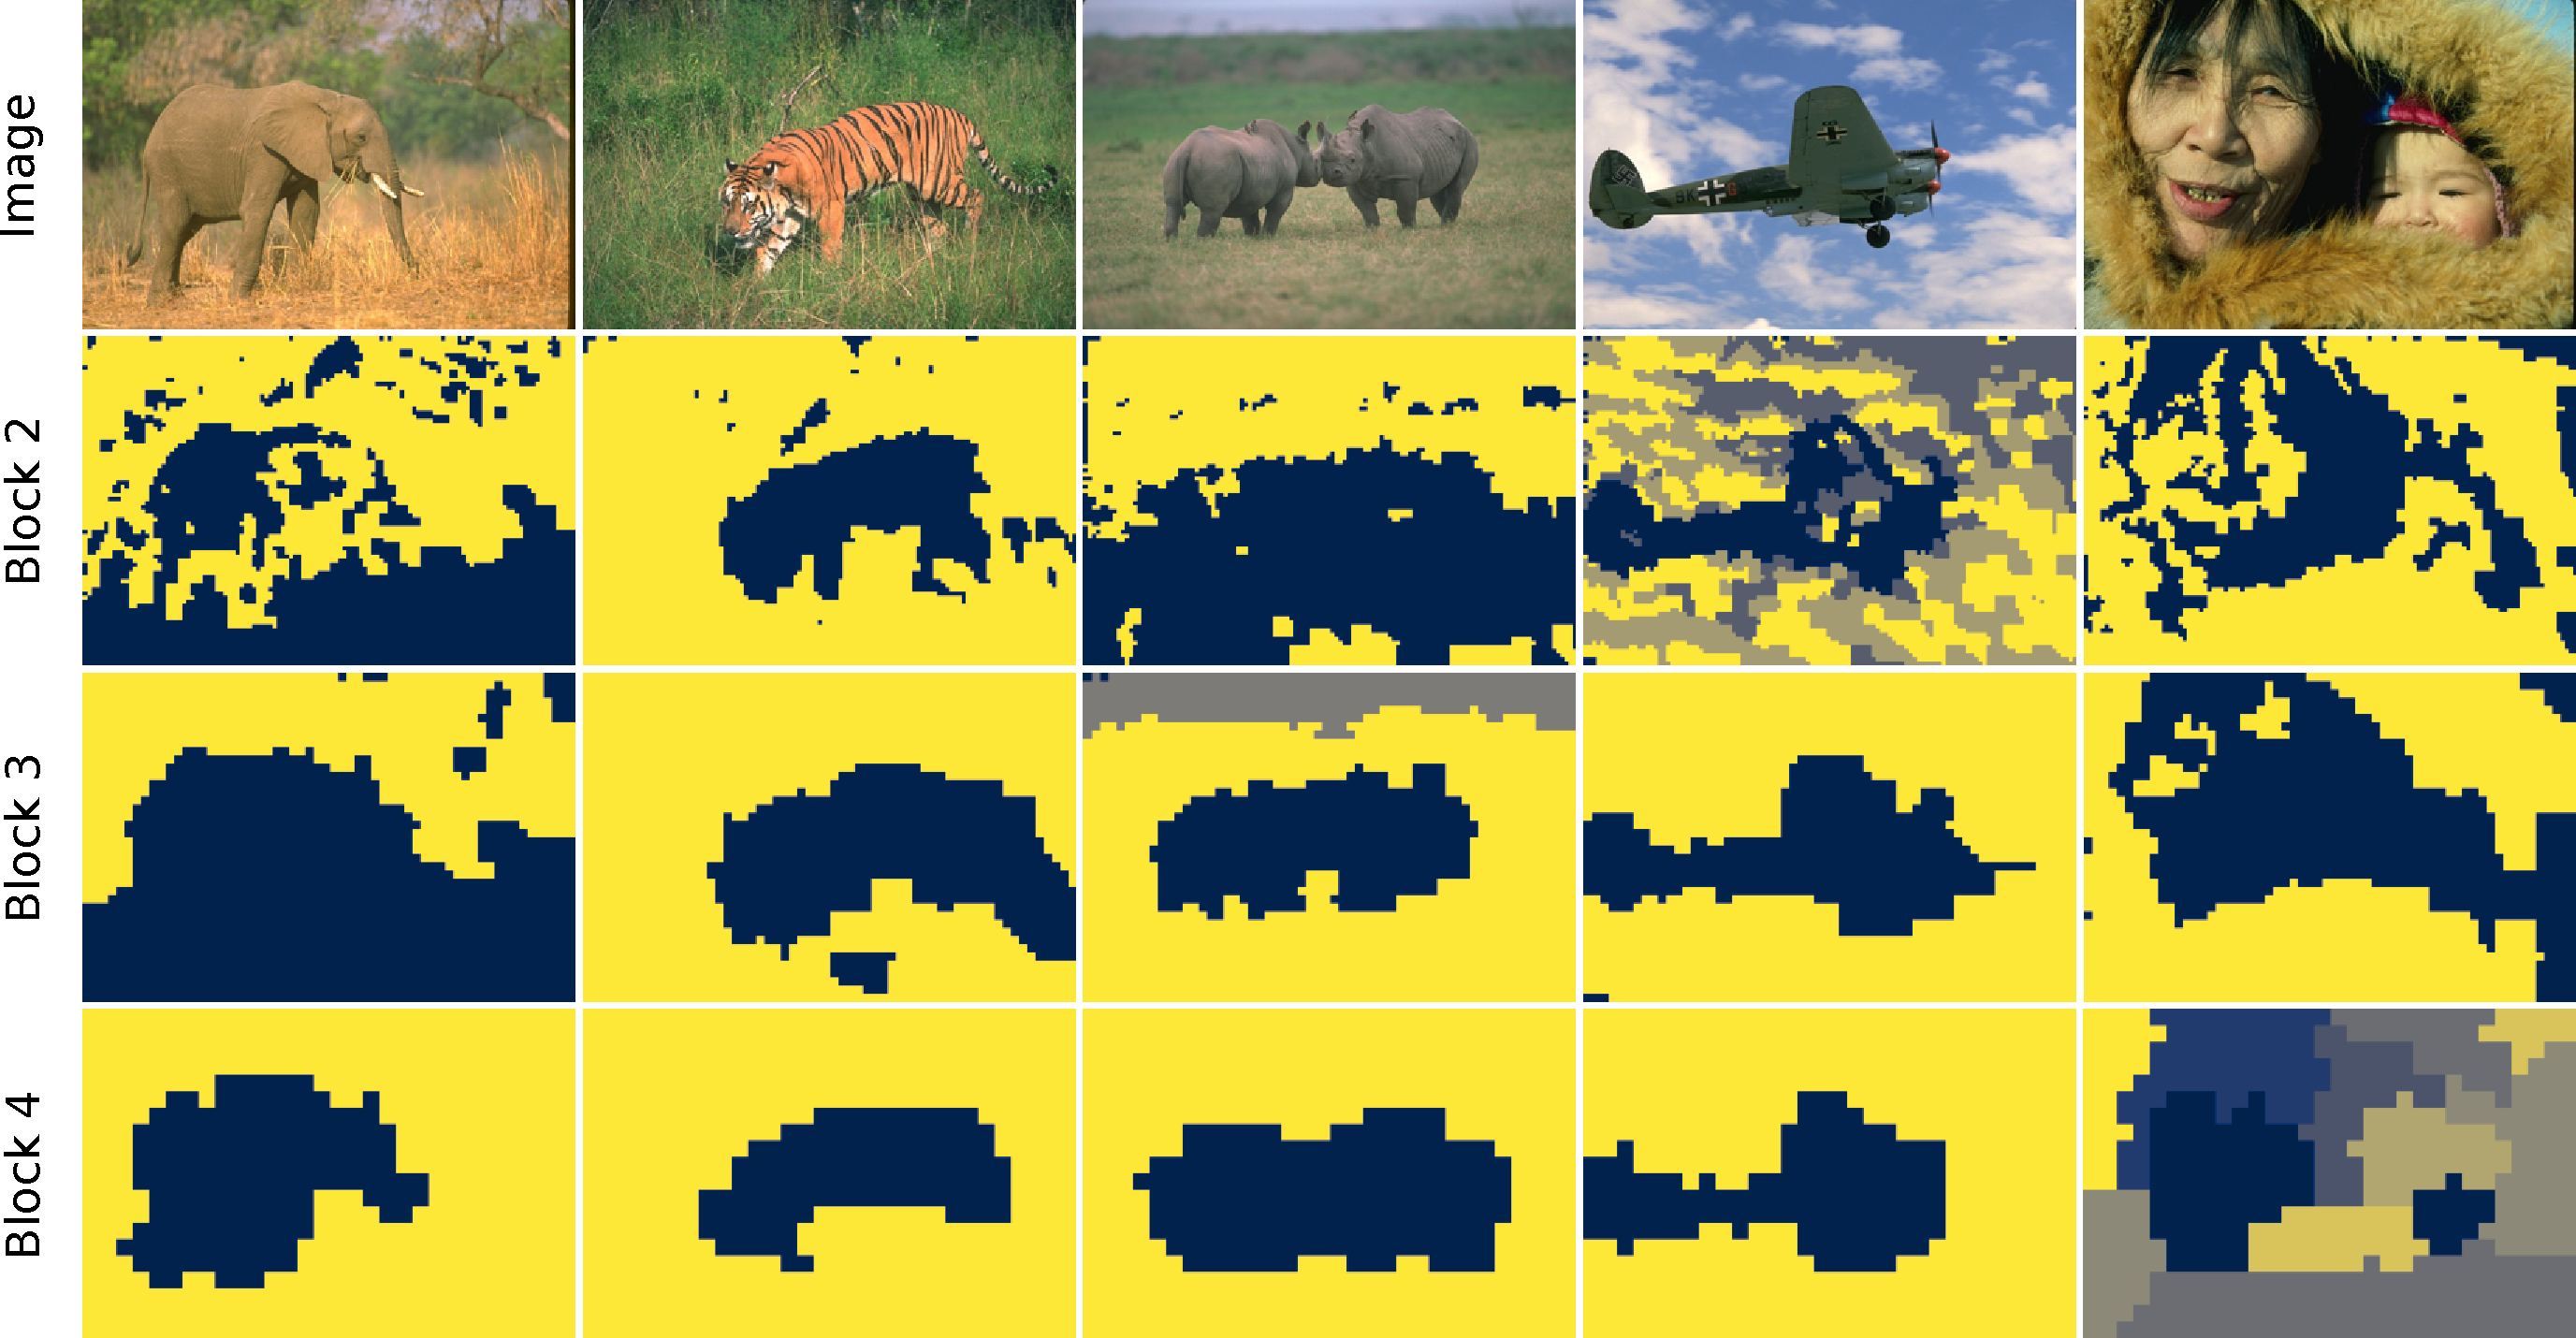
\includegraphics[width=\textwidth]{figures/fslic_sfcm_bsd500.pdf}
    \caption{The segmentation results of six images from BSD500 using the feature superpixel-based clustering approach.}
    \label{fig:fslic_sfcm_bsd500}
\end{figure}

\autoref{fig:fslic_sfcm_bsd500} shows the segmentation results obtained on six images from BSD500 at different depths of the model. The figure shows that the results obtained from the shallower layers are either under- or over-segmented. This is likely due to the network extracting more general features at the early layers. In comparison, most of the segmentation results from block 4 show that the model was able to separate the different real-world objects found in the original images. Feature images extracted from deeper layers contain rich semantic information due to their increased number of feature maps. Nevertheless, some of the regions in the segmentation masks have weak boundary adherence.


\subsection{Clustering Feature Pixels}

The second segmentation experiment investigated clustering the pixels of the feature images directly using k-means. Just as in the previous experiment, the number of clusters was chosen according the silhouette method, where the search range was set to $[2, 10]$. \autoref{fig:bsd500_results} shows the results obtained from this experiment. By looking at the figure, we can see that the model tends to extract more general features in the shallower layers. For example, the results from block 2 separate the pixels in the image based on brightness uniformity. In comparison, the results from block 4 are able to separate the real-world objects in the image on a more abstract level. This indicates that the foreground pixels are well-separated from the background pixels in the latent space of the model. Compared to the previous experiment, the results from block 4 have a stronger boundary adherence. This can be attributed to the smaller regions covered by the feature pixels compared to those covered by the feature superpixels. As a result, the feature pixels are less likely covering more than one object. Therefore, they are sufficiently isolated from each other in the feature space and can easily be clustered in the subsequent step.

\begin{figure}[thbp]
    \centering
    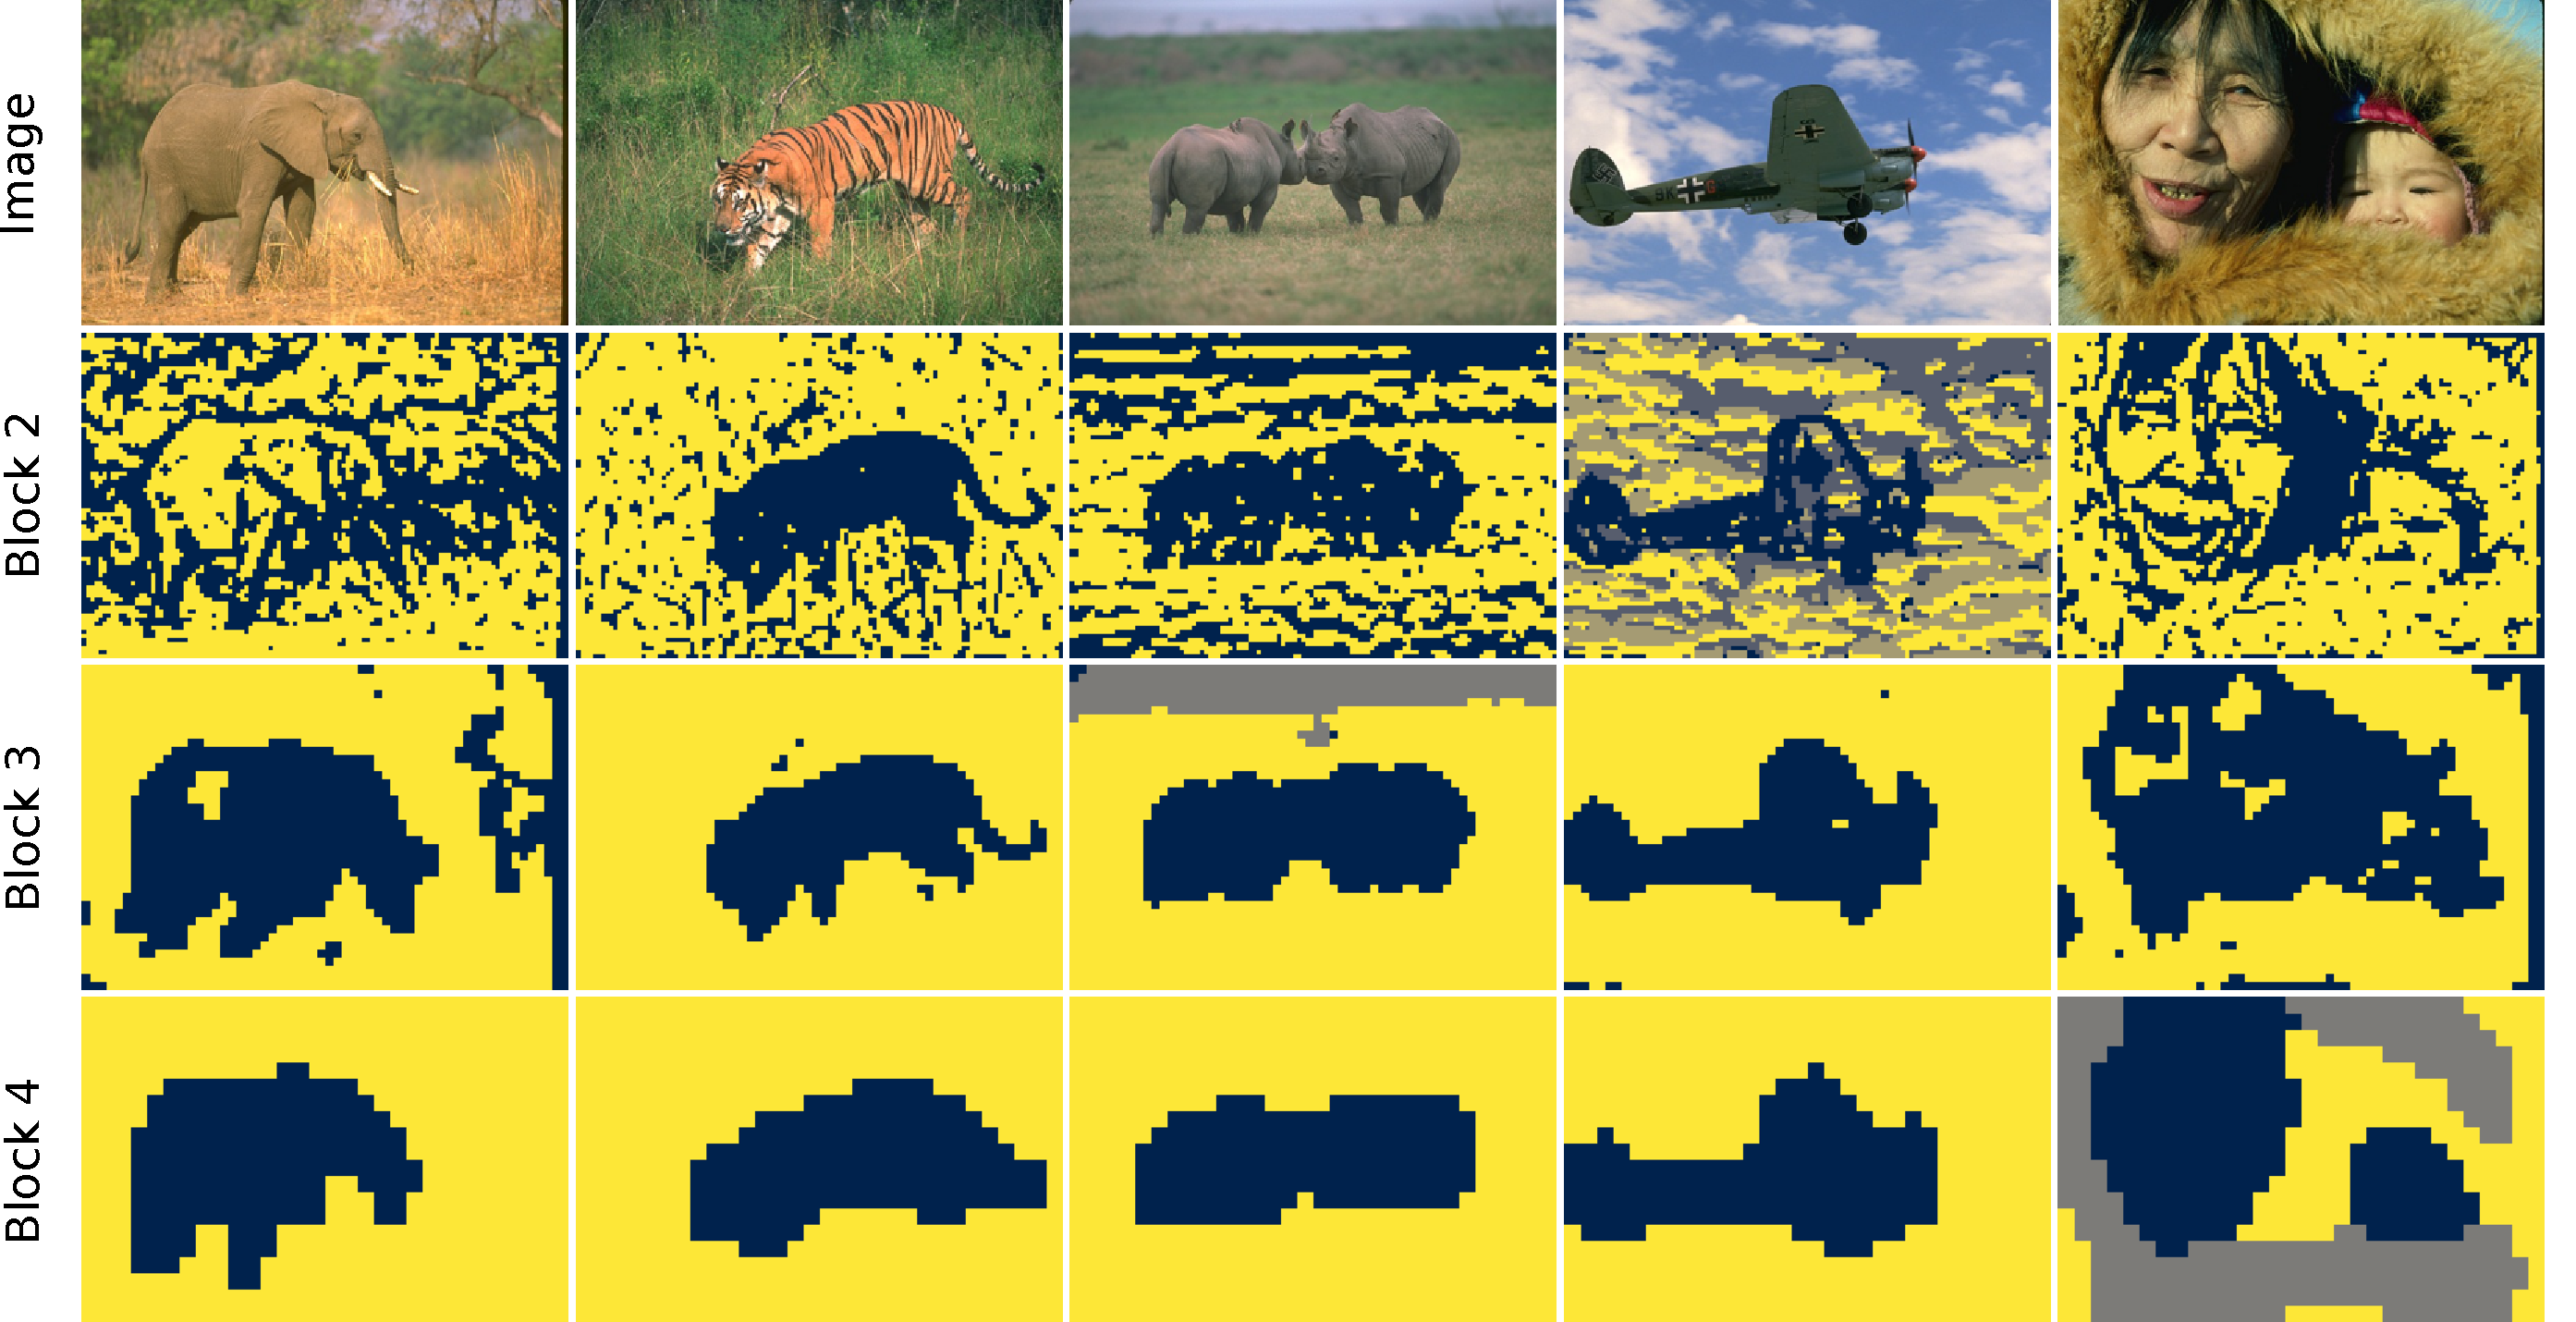
\includegraphics[width=\textwidth]{figures/bsd500_results.pdf}
    \caption{The segmentation results of six images from BSD500 using the feature pixel clustering approach.}
    \label{fig:bsd500_results}
\end{figure}

\begin{figure}[thbp]
    \centering
    \includegraphics[width=\textwidth]{figures/cityscapes_results.pdf}
    \caption{A figure showing the results obtained after processing six images from Cityscapes using the feature pixel clustering approach.}
    \label{fig:cityscapes_results}
\end{figure}

This experiment also investigated segmenting images from the Cityscapes dataset. Since images from Cityscapes contain more objects than images from BSD500, the silhouette method interval was changed to $[2, 40]$. \autoref{fig:cityscapes_results} shows the obtained segmentation masks. Despite the increased range, only two clusters were found in the results from blocks 2, 3 and 4. The segmentations masks obtained at block 4 show that multiple real-world objects are grouped into one cluster. However, as we saw in the previous section (see \autoref{fig:pca_images_weird}), the objects in the image are indeed separated in the feature space of the model. This suggests that the silhouette index may not be appropriate for choosing the cluster number in more complex images. Concerning the masks obtained from block 2 and 3, the clusters obtained separate the objects in the image according to two global features. The cluster indicated by the blue region represents the boundaries present in the image. These are regions with a sharp change in contrast. However, the yellow cluster represents non-boundary objects characterized by a more homogeneous color and less texture variation. It includes smooth objects such as the sky, the road and the sidewalk.



\section{Feature Map Analysis}\label{section:further_analysis}



In this section, we analyze feature map similarities and differences between the objects in the foregrounds of multiple images. First, we construct two semantically different classes of images. Then, the segmentation masks of the images are obtained using the k-means-based approach discussed in the previous section. Lastly, we compare the intra-class and inter-class distributions of the feature map values in the clusters corresponding to the objects in the foreground. 

More formally, let $C$ represent a class of semantically similar images, which all contain similar foreground objects. Then, every image $I \in C$ can be viewed as a function which maps a pixel's 2D position $p$ to an RGB color $I(p)$. The corresponding feature image of $I$ is obtained by extracting its features from the VGG16 model. We refer to the feature image as $\text{VGG}[I]$, which can also be viewed as function which maps a pixel $p$ to its feature representation $\text{VGG}[I](p)$. The features of a pixel are represented by a $d$-dimensional vector $\text{VGG}[I](p)=(f_p^{(0)}, \ldots, f_p^{(d-1)})$. After extracting the feature image, the segmentation mask is obtained by clustering the feature pixels into coherent groups. We refer to the set of feature pixels representing the foreground objects in the mask as $G(I)$. In this section, we analyze the distributions of the feature maps of the pixels in $G(I)$. We define the $k$-th feature map of the foreground clusters to be the set consisting of the $k$-th entry of the feature pixels in $G(I)$:
\begin{equation}
    M^{(k)}\!(I) = \{f_p^{(k)} : \forall p \in \mathbb{Z}^2, \text{VGG}[I](p) \in G(I) \}.
\end{equation}

\subsubsection{Distribution Similarity}

In order to quantitatively analyze multiple distributions, a similarity score needs to be calculated. The \emph{Kolmogorov-Smirnov} (KS) test \parencite{massey1951kolmogorov} is a widely used non-parametric test of goodness of fit. It can be used to compare the empirical cumulative distribution functions (ECDFs) of two samples. The ECDF of a sample $S$ is defined as \parencite{massey1951kolmogorov}:
\begin{equation}
    F(x | S) = \frac{|\{s: s \in S, s \le x\}|}{|S|}.
\end{equation}
In other words, $F(x | S)$ measures the fraction of the elements in the sample which are less than or equal to $x$.
Given two samples, $S_1$ and $S_2$, the KS test reports a score of the dissimilarity between the sample distributions. The test measures the maximum vertical distance between the two overlayed ECDFs of the samples. It is defined as:
\begin{equation}
    \text{KS}(S_1, S_2) = \max_x |F(x | S_1) - F(x | S_2)|.
\end{equation}
Two similar ECDFs will have a lower KS score than two dissimilar ones.

In our analysis, we need to compare multiple distributions with each other. Hence, we propose computing an aggregated score based on the KS test. Let $C_1$ and $C_2$ represent two sets of images. The $\Delta$-score measures the dissimilarity between the feature map distributions of the two classes. It is calculated as follows:
\begin{equation}
    \Delta_{k,l}(C_1, C_2) = \frac{\sum_{I \in C_1}{\max_{I' \in C_2} \text{KS}(M^{(k)}\!(I), M^{(l)}\!(I'))}}{|C_1|}.
    \label{eq:delta}
\end{equation}
The smaller the $\Delta$-score, the greater the similarity between the $k$-th feature maps of $C_1$ with respect to the $l$-th feature maps of $C_2$. However, $\Delta_{k,l}(C_1, C_2)$ is not necessarily equal to $\Delta_{l,k}(C_2, C_1)$. In order to accommodate for this, we average over both values:
\begin{equation}
    \bar{\Delta}_{k,l}(C_1, C_2) = \frac{1}{2} (\Delta_{k,l}(C_1, C_2) + \Delta_{l,k}(C_2, C_1)).
    \label{eq:h_score}
\end{equation}
Therefore, the $\bar{\Delta}$-score can yield a symmetric score for comparing the feature maps of two classes of images. The greater the value of the $\bar{\Delta}$-score, the greater the dissimilarity between the distributions of the two feature maps in question.

\autoref{fig:classes} shows the segmentation masks obtained from two subsets of BSD500 containing semantically similar images. The class representing images of horses (a-e) is semantically different from the class representing images of bears (f-j). In what follows, we refer to the two classes of images as $C_{\text{horses}}$ and $C_{\text{bears}}$.

\begin{figure}[t]
    \centering
        \centering
        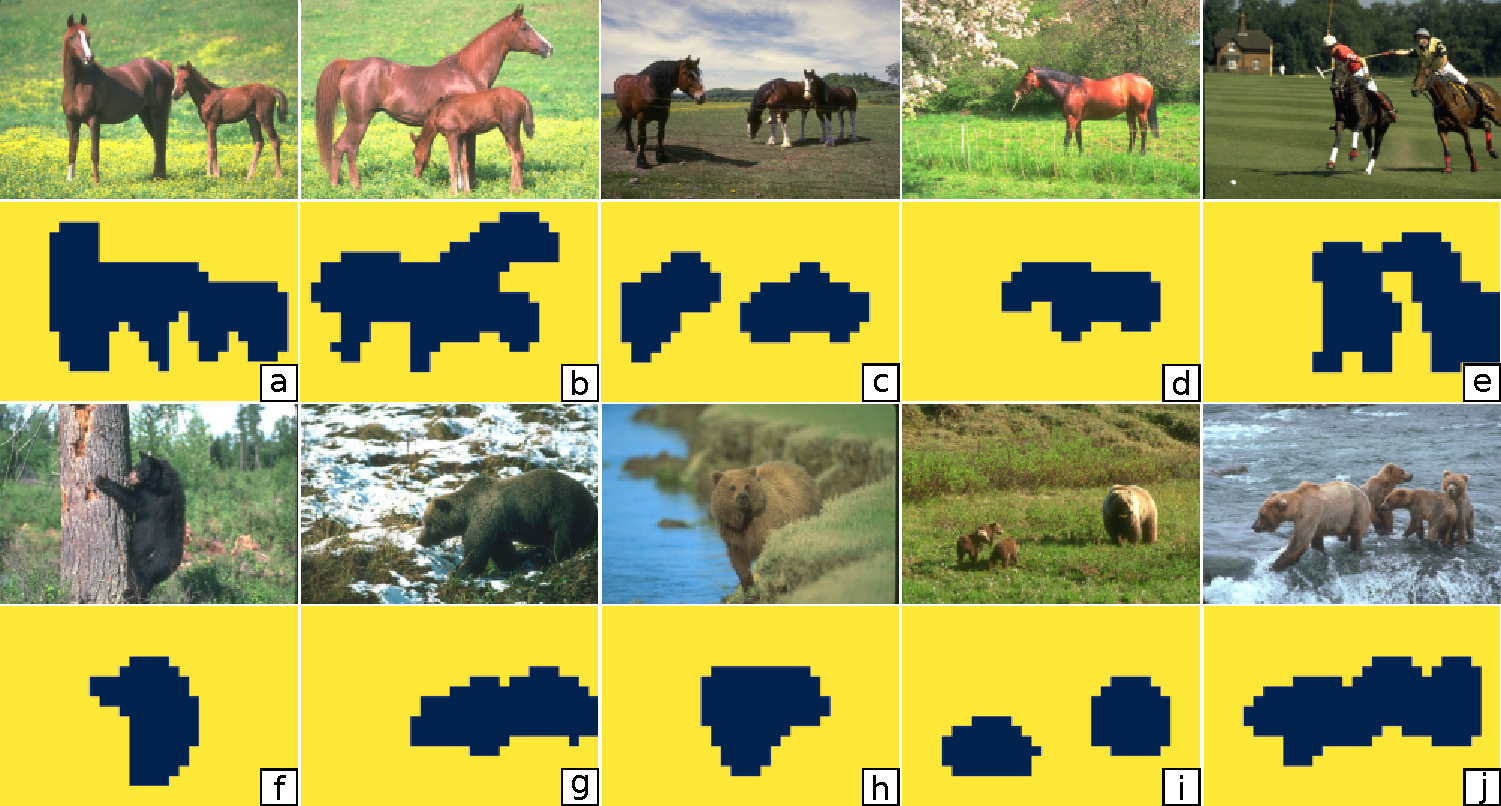
\includegraphics[width=\textwidth]{figures/classes.pdf}
    \caption{Two classes of similar images from BSD500 and their segmentation masks.}
    \label{fig:classes}
\end{figure}


\subsection{Class-Centric Analysis}

Different feature maps can capture different pieces of semantic information. In this subsection, we compare the distributions of single feature maps on an intra- and inter-class level.

\subsubsection{Intra-Class Comparison}

The aforementioned $\bar{\Delta}$-score can be adopted to calculate the dissimilarity of the intra-class single feature map distributions:
\begin{equation}
    \Sigma_k(C) = \bar{\Delta}_{k,k}(C, C).
    \label{eq:E}
\end{equation}
The $\Sigma_k$-score measures the distribution of the $k$-th feature map among the feature clusters in one class. Feature maps with a lower $\Sigma$-score report the similarities between the class clusters while those with larger $\Sigma$-score highlight the clusters' differences.

\autoref{fig:barcharts} shows a chart of the 12 feature maps with lowest and highest $\Sigma(C_{\text{horses}})$-scores (the ECDFs are shown in \autoref{fig:ecdfs}). The left (right) bar chart represents the dimensions with the greatest distribution similarity (dissimilarity).
\begin{figure}[t]
    \centering
    \begin{subfigure}{.49\textwidth}
        \centering
        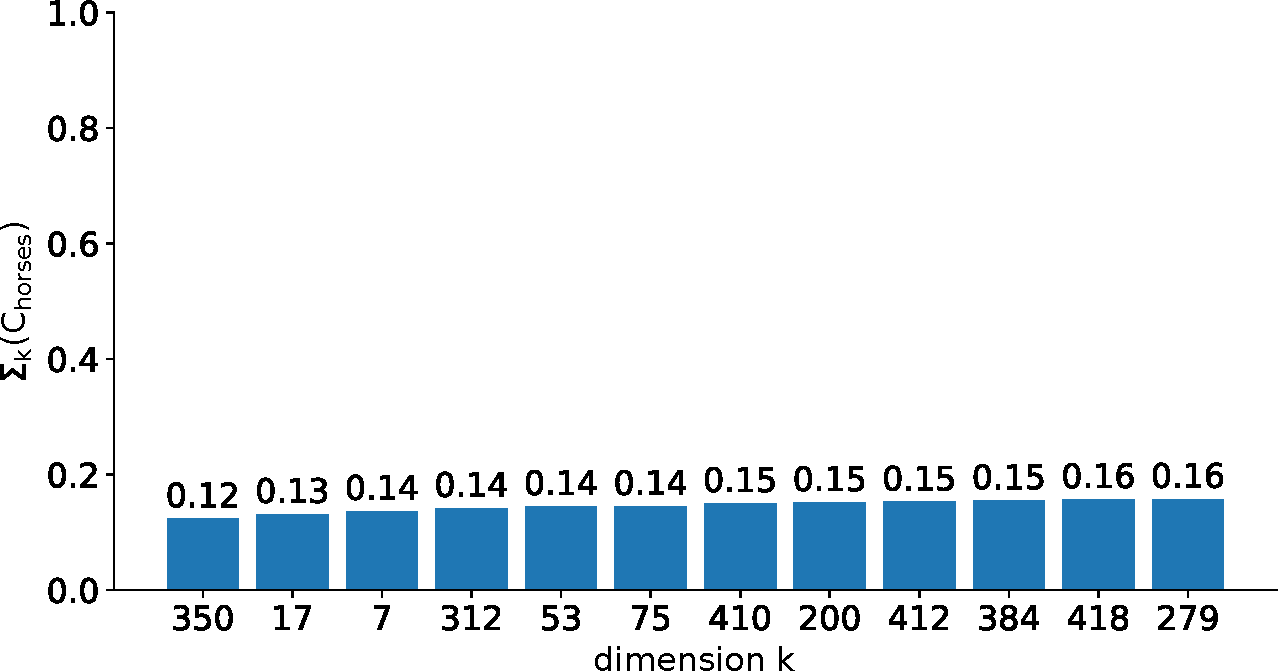
\includegraphics[width=\linewidth]{figures/lowest_scores_barchart_ds15.pdf}
    \end{subfigure}
    \hfill
    \begin{subfigure}{.49\textwidth}
        \centering
        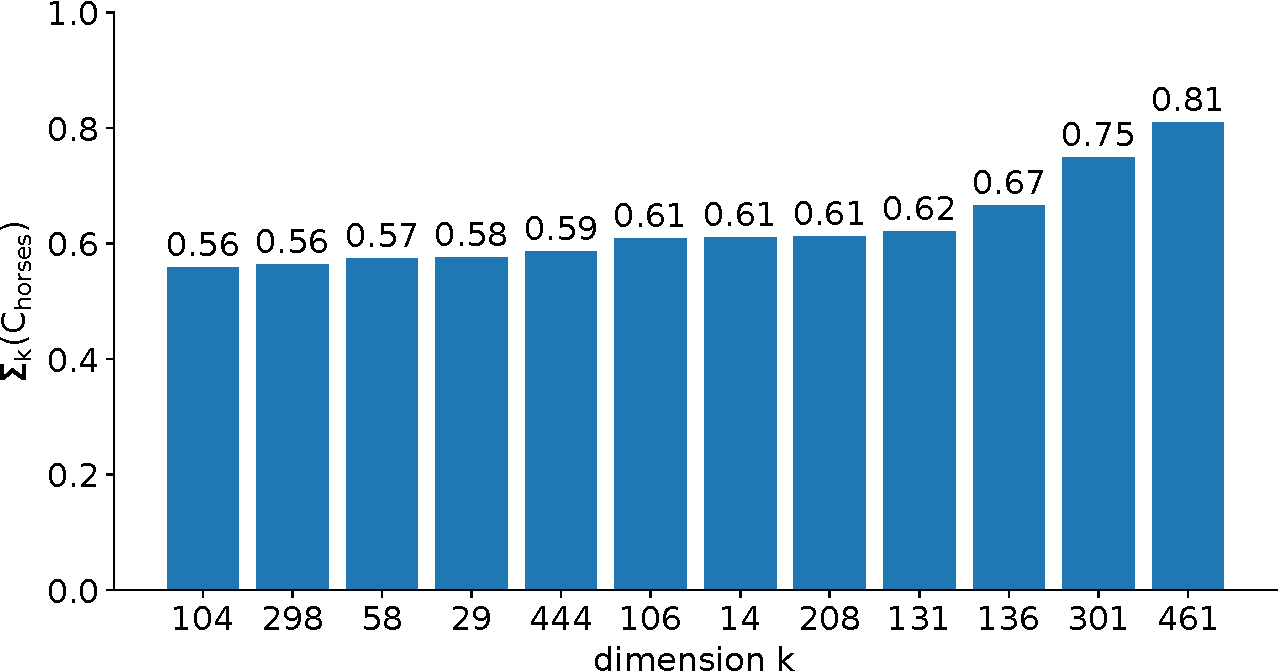
\includegraphics[width=\linewidth]{figures/highest_scores_barchart_ds15.pdf}
    \end{subfigure}
    \caption{A figure showing the 12 dimensions with the lowest $\Sigma$-scores (left) and the highest $\Sigma$-scores (right) in $C_{\text{horses}}$.}
    \label{fig:barcharts}
\end{figure}
This is further supported by the parallel coordinate plots (PCPs) of the dimensions shown in \autoref{fig:pcp_similar} and \autoref{fig:pcp_dissimilar}. 

The PCPs of \autoref{fig:pcp_similar} show that the model contains a feature subspace where the foreground feature clusters of the images in $C_{\text{horses}}$ are similarly distributed. The distributions of the foreground clusters appear to be unimodal with similar means and variances. In addition to that, the correlation matrices shown on the right-hand side of the figure have similar values.

In comparison, the PCPs shown in \autoref{fig:pcp_dissimilar} show the feature maps which are very dissimilarly distributed. The feature maps appear to have different means and variances across the different clusters (f-j). Moreover, the correlation matrices of the feature maps bear little to no similarity.

\begin{sidewaysfigure}
    \centering
    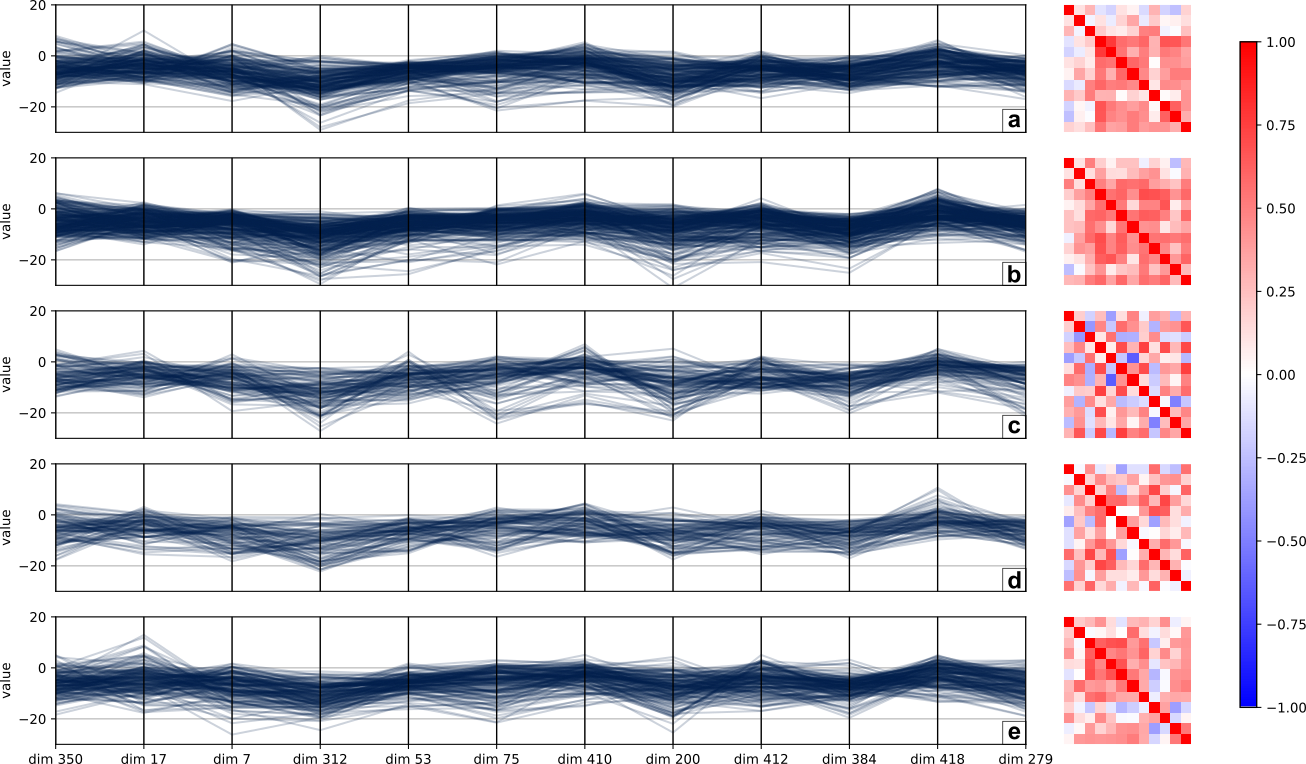
\includegraphics[width=\textheight]{figures/PCP_similar.png}
    \caption{Five images of horses from BSD500 are segmented using the pipeline described in Chapter \ref{chapter:clustering_in_feature_space}. The feature vectors in the blue cluster of each segmentation result shown in \autoref{fig:classes} (a-e) are analyzed. The parallel coordinates plot shows the vectors of their corresponding cluster in the 12 dimensions with the lowest $\Sigma$-scores (see \autoref{eq:E}). The correlation matrix of the dimensions (in their displayed order) is shown on the right.}
    \label{fig:pcp_similar}
\end{sidewaysfigure}

\begin{sidewaysfigure}
    \centering
    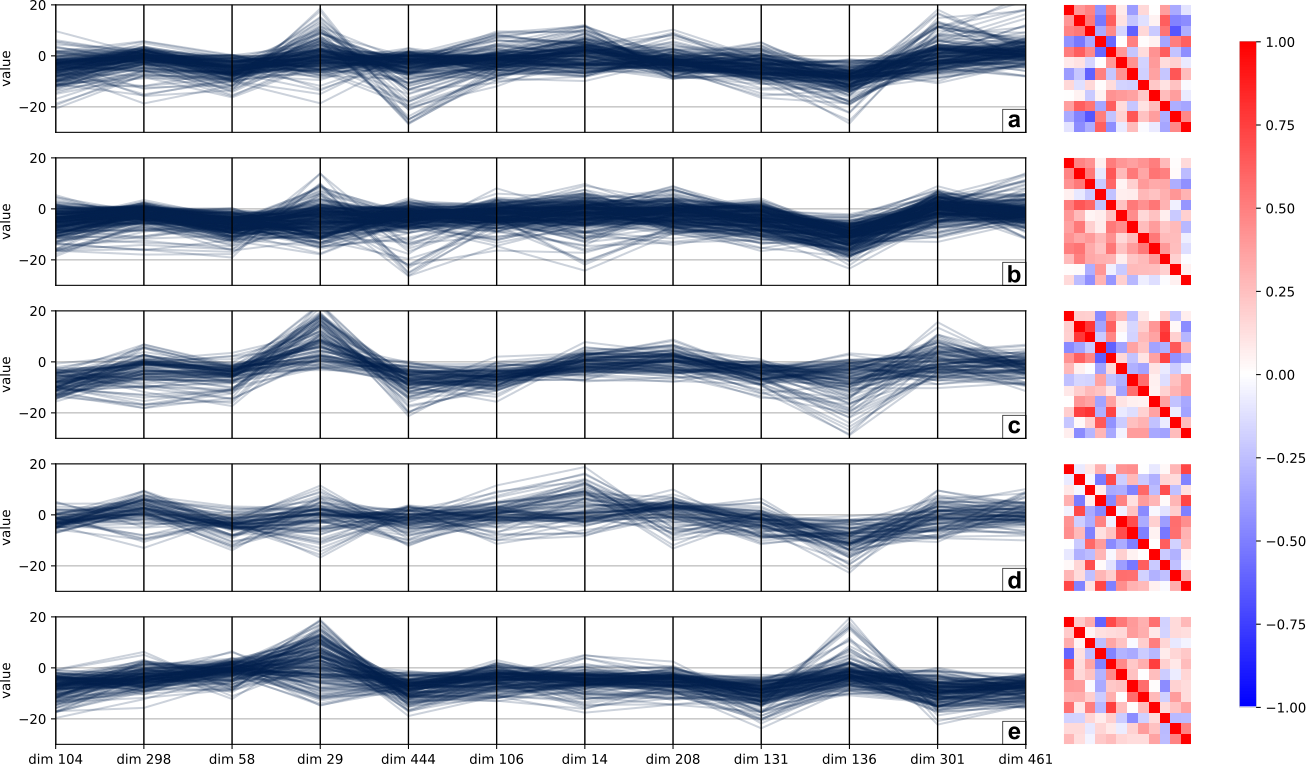
\includegraphics[width=\textheight]{figures/PCP_dissimilar.png}
    \caption{Five images of horses from BSD500 are segmented using the pipeline described in Chapter \ref{chapter:clustering_in_feature_space}. The feature vectors in the blue cluster of each segmentation result shown in \autoref{fig:classes} (a-e) are analyzed. The parallel coordinates plot shows the vectors of the corresponding cluster in the 12 dimensions with the highest $\Sigma$-scores (see \autoref{eq:E}). The correlation matrix of the dimensions (in their displayed order) is shown on the right.}
    \label{fig:pcp_dissimilar}
\end{sidewaysfigure}

The next step of the analysis involved overlaying a heat map of the aforementioned feature maps onto the original images. This would reveal the similarities and differences that the model finds among the different images in one class. In order to superimpose the feature maps onto the original images, the feature maps need to be upsampled to the original spatial resolution of the images. This was achieved by employing nearest neighbor upsampling.


\autoref{fig:overlay_similar_dims} shows the upsampled feature maps of the five dimensions with the lowest $\Sigma$-scores superimposed on the original images. By looking at the figure, we can identify similarities in the feature maps across the different images. For example, the feature maps of dimension 350 are positively valued in the areas covering the top part of the horses shown.

\begin{figure}[!t]
    \centering
    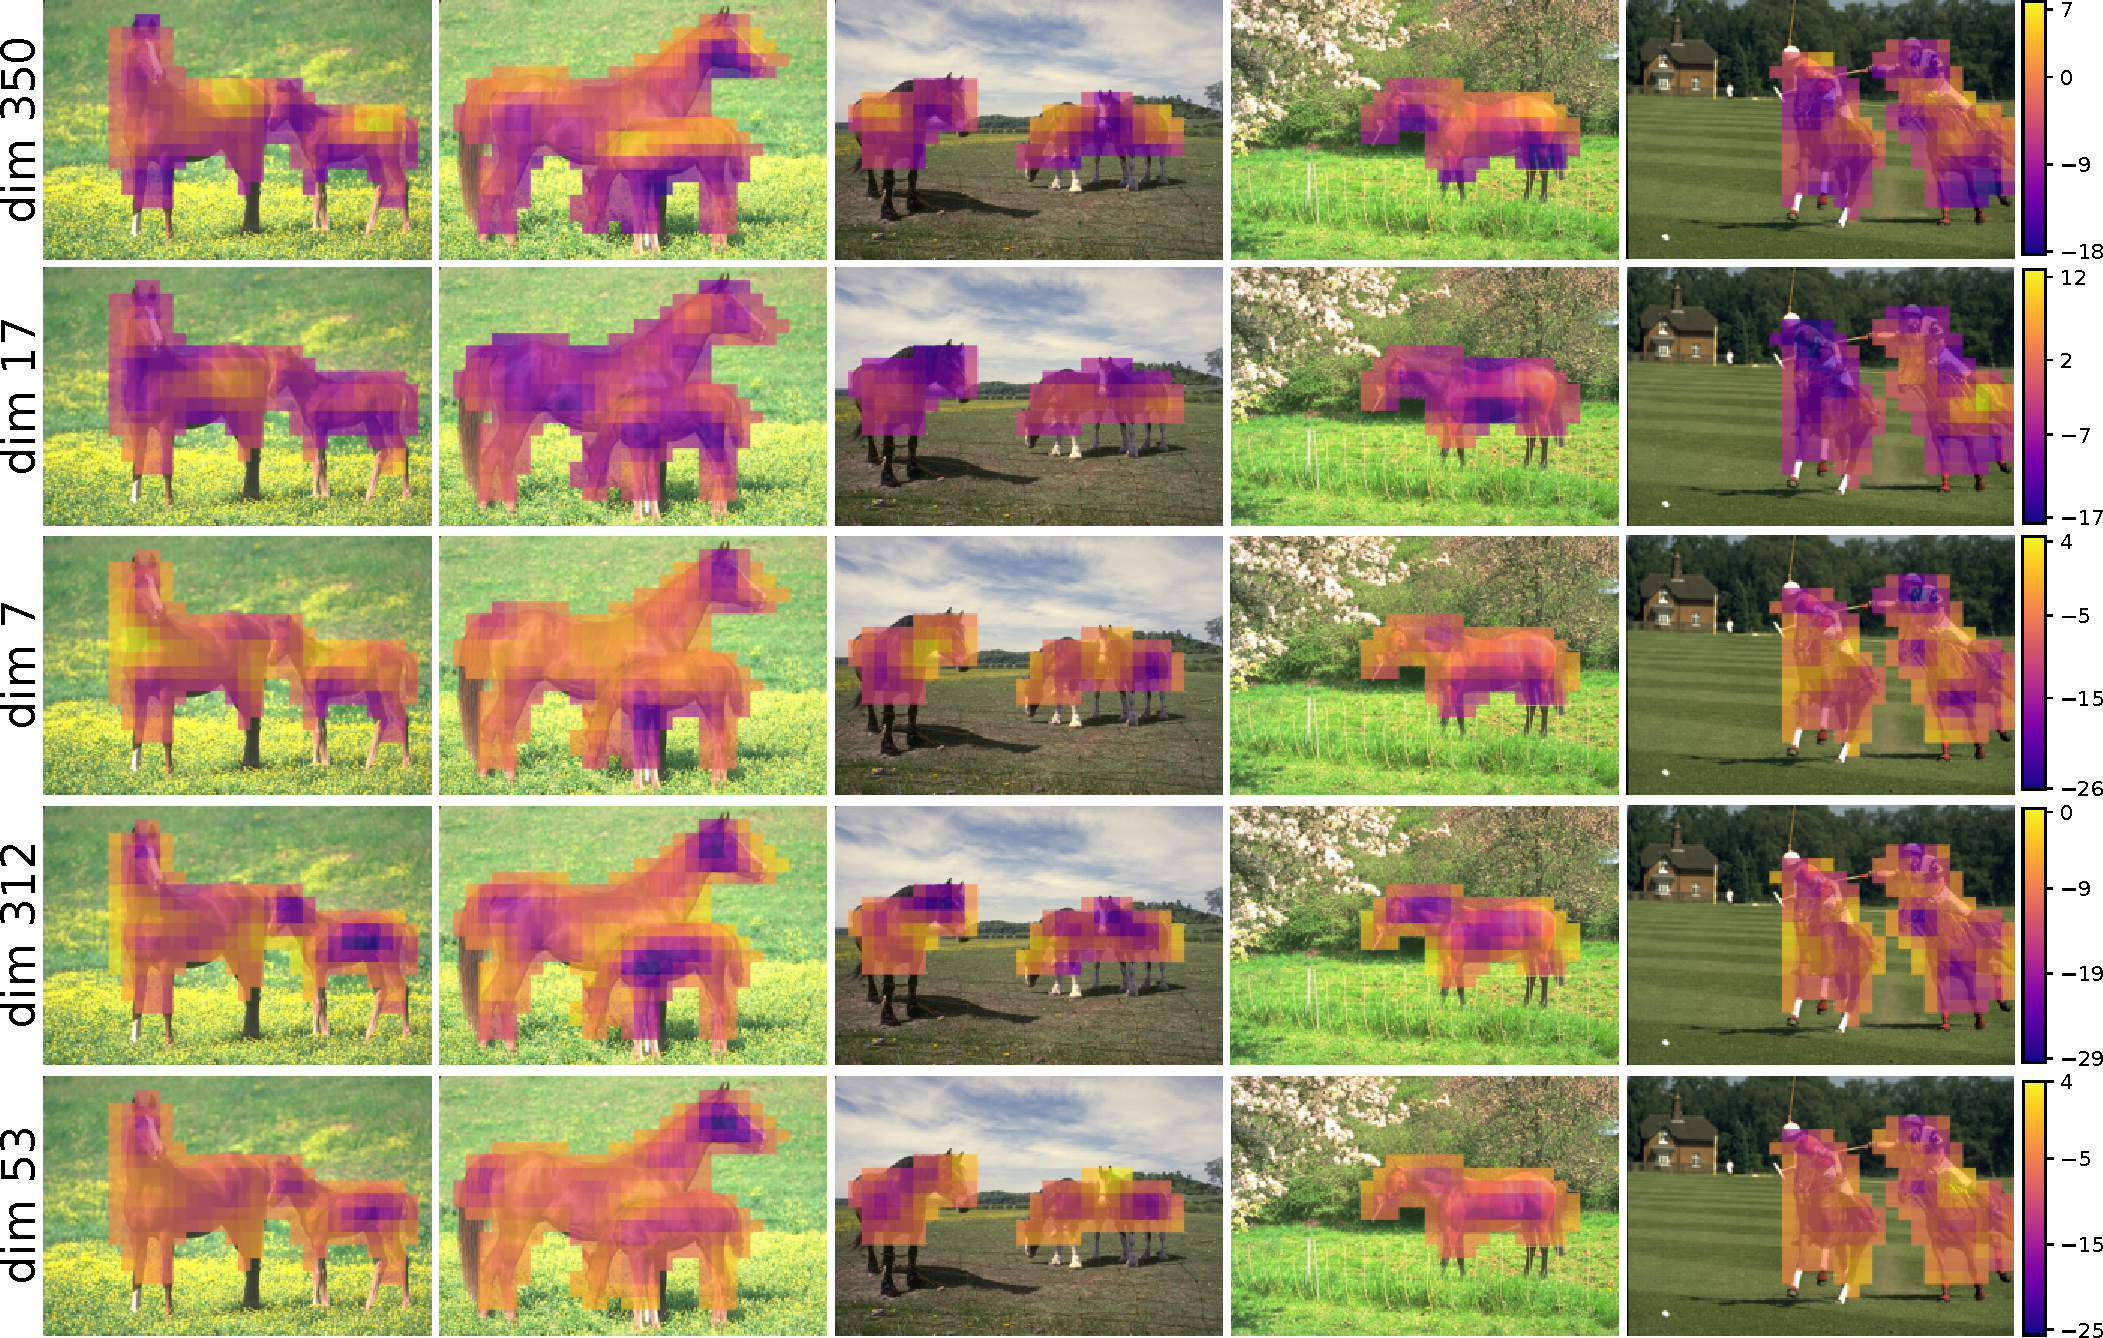
\includegraphics[width=.9\textwidth]{figures/overlayed_dim_similar.pdf}
    \caption{The five lowest $\Sigma(C_{\text{horses}})$-scoring feature maps superimposed on their images.}
    \label{fig:overlay_similar_dims}
\end{figure}

We also applied the same procedure to observe the feature maps that can discriminate between the objects. \autoref{fig:overlay_dissimilar_dims} shows the feature maps of the five highest $\Sigma$-scoring feature maps superimposed on the original images. The figure shows that the model can differentiate between the clusters based on the presence or absence small-scale object parts. For instance, the feature map of dimension 208 has a high activation for the area covering the tail of the horse. This explains the images where the tail of the horse is not clearly visible having low feature map activations. Similarly, the feature map of dimension 136 has a greater value for the area covering the only horse-rider in the rightmost image.

\begin{figure}[!t]
    \centering
    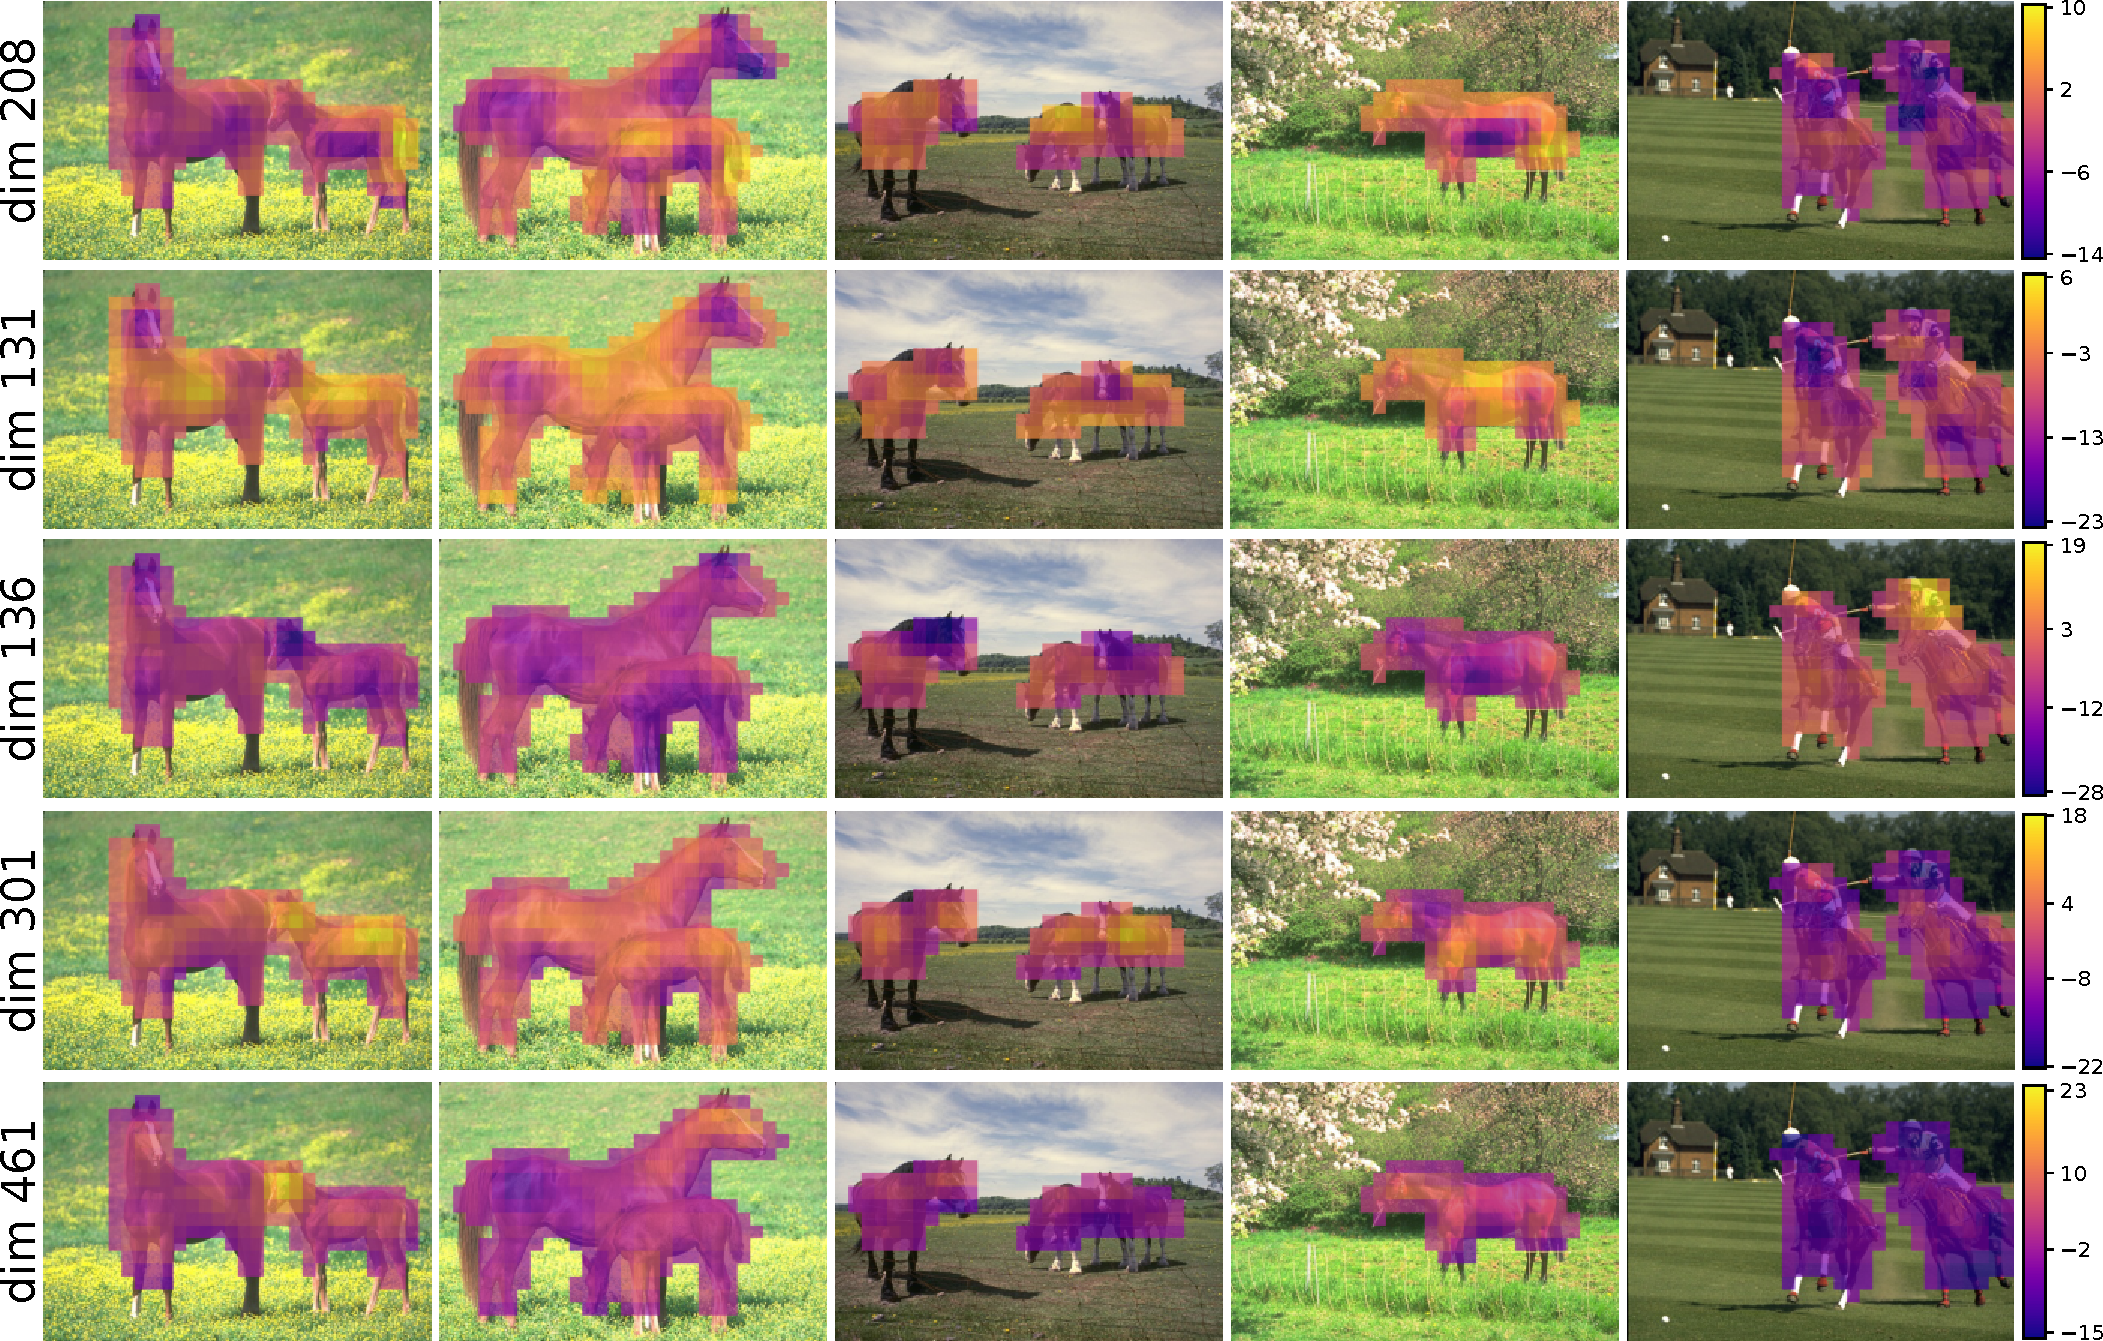
\includegraphics[width=.9\textwidth]{figures/overlayed_dim_dissimilar.pdf}
    \caption{The five highest $\Sigma(C_{\text{horses}})$-scoring feature maps superimposed on their images.}
    \label{fig:overlay_dissimilar_dims}
\end{figure}

A similar intra-class analysis process was conducted for $C_{\text{bears}}$. The results obtained are shown in \autoref{appendix:s_bears_analysis} of \autoref{chapter:experiment_details}.

\subsubsection{Inter-Class Comparison}

The next part of our analysis process focused on ranking the feature maps based on their distribution (dis-)similarity among two classes. The $\bar{\Delta}$-score from \autoref{eq:h_score} can be adopted for calculating the distribution dissimilarity of a feature map in one class with respect to the same feature map in another class:
\begin{equation}
    \Gamma_{k}(C_1, C_2) = \bar{\Delta}_{k, k}(C_1, C_2).
    \label{eq:F}
\end{equation}
A small $\Gamma$-score reports a feature map which captures similar semantic information found in the images of $C_1$ and $C_2$.

\autoref{fig:pairplot} shows a matrix plot of the $\Sigma$-scores and $\Gamma$-scores of $C_{\text{horses}}$ and $C_{\text{bears}}$. As the figure shows, the three measures seem to have unimodal distributions. Furthermore, the PCP on the right can be used to retrieve feature maps which can differentiate between images from $C_\text{horses}$ and $C_{\text{bears}}$. For example, the red line in the PCP which represents feature map 130 has a low value for $\Sigma(C_\text{bears})$, but a larger value for $\Sigma(C_\text{horses})$ and $\Gamma(C_{\text{horses}}, C_{\text{bears}})$. The feature map can be used to differentiate between images of the two classes since it is has a low intra-class distribution and large inter-class distribution. As shown in \autoref{fig:overlayed_differentiator}, the feature map is only activated on areas covering the head of the horse. However, the areas covering the bears have uniform low activations. In future work, interactive filtering of the feature maps shown in the PCP could be used to gain a deeper insight of the class similarities and differences. For example, selecting the feature maps with a low $\Sigma$-score and a large $\Gamma$-score could reveal unique attributes found in one class but not in the other class.

\begin{figure}
    \centering
    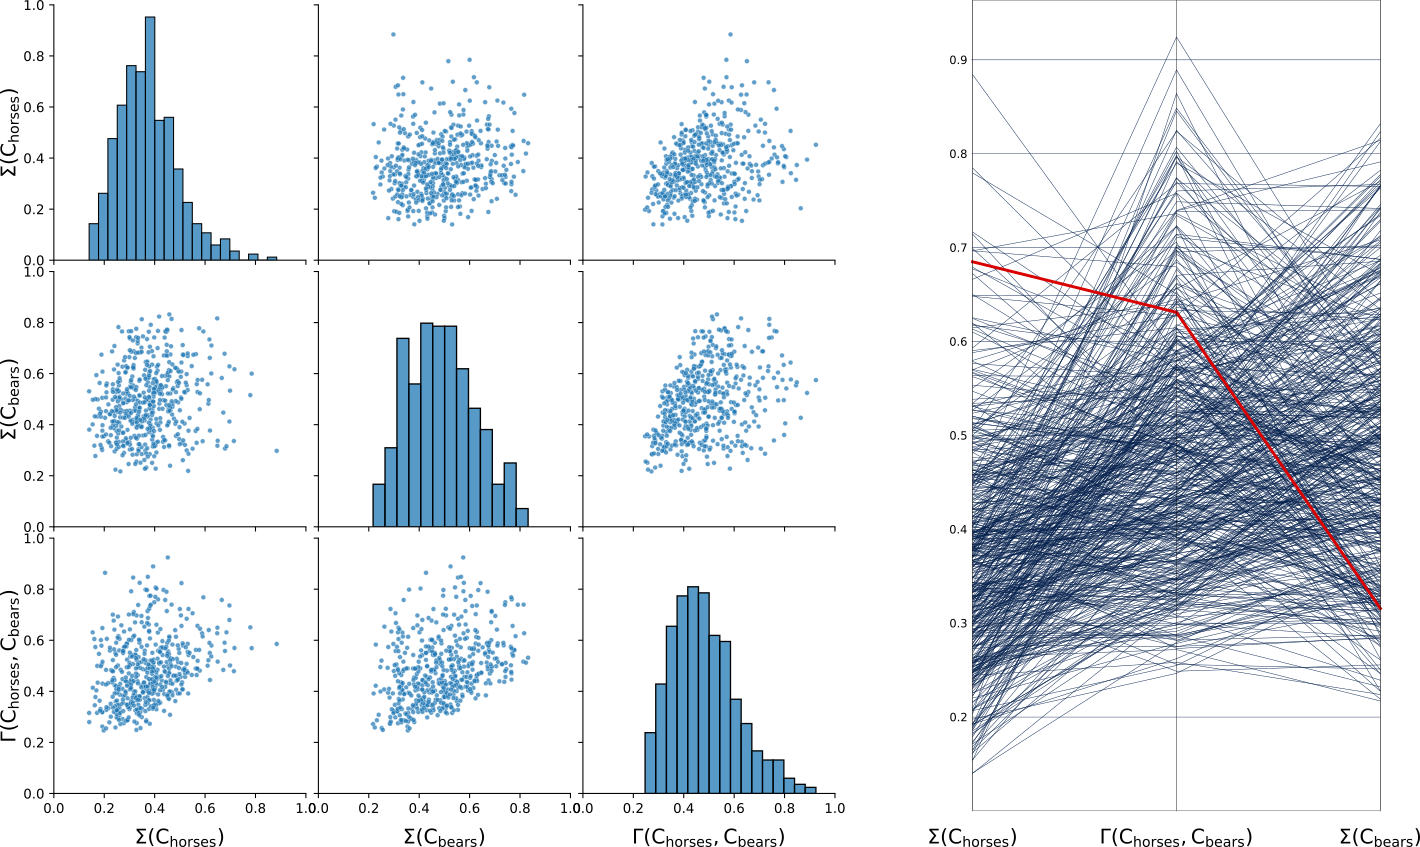
\includegraphics[width=\textwidth]{figures/pairplot.png}
    \caption{A matrix plot (left) showing the relationship between $\Sigma(C_{\text{horses}})$, $\Sigma(C_{\text{bears}})$ and $\Gamma(C_{\text{horses}}, C_{\text{bears}})$. Each line in the PCP (right) represents one feature map. The red line has low $\Sigma(C_{\text{bears}})$ and high $\Gamma(C_{\text{horses}}, C_{\text{bears}})$. The feature map is shown in \autoref{fig:overlayed_differentiator}.}
    \label{fig:pairplot}
\end{figure}

\begin{figure}
    \centering
    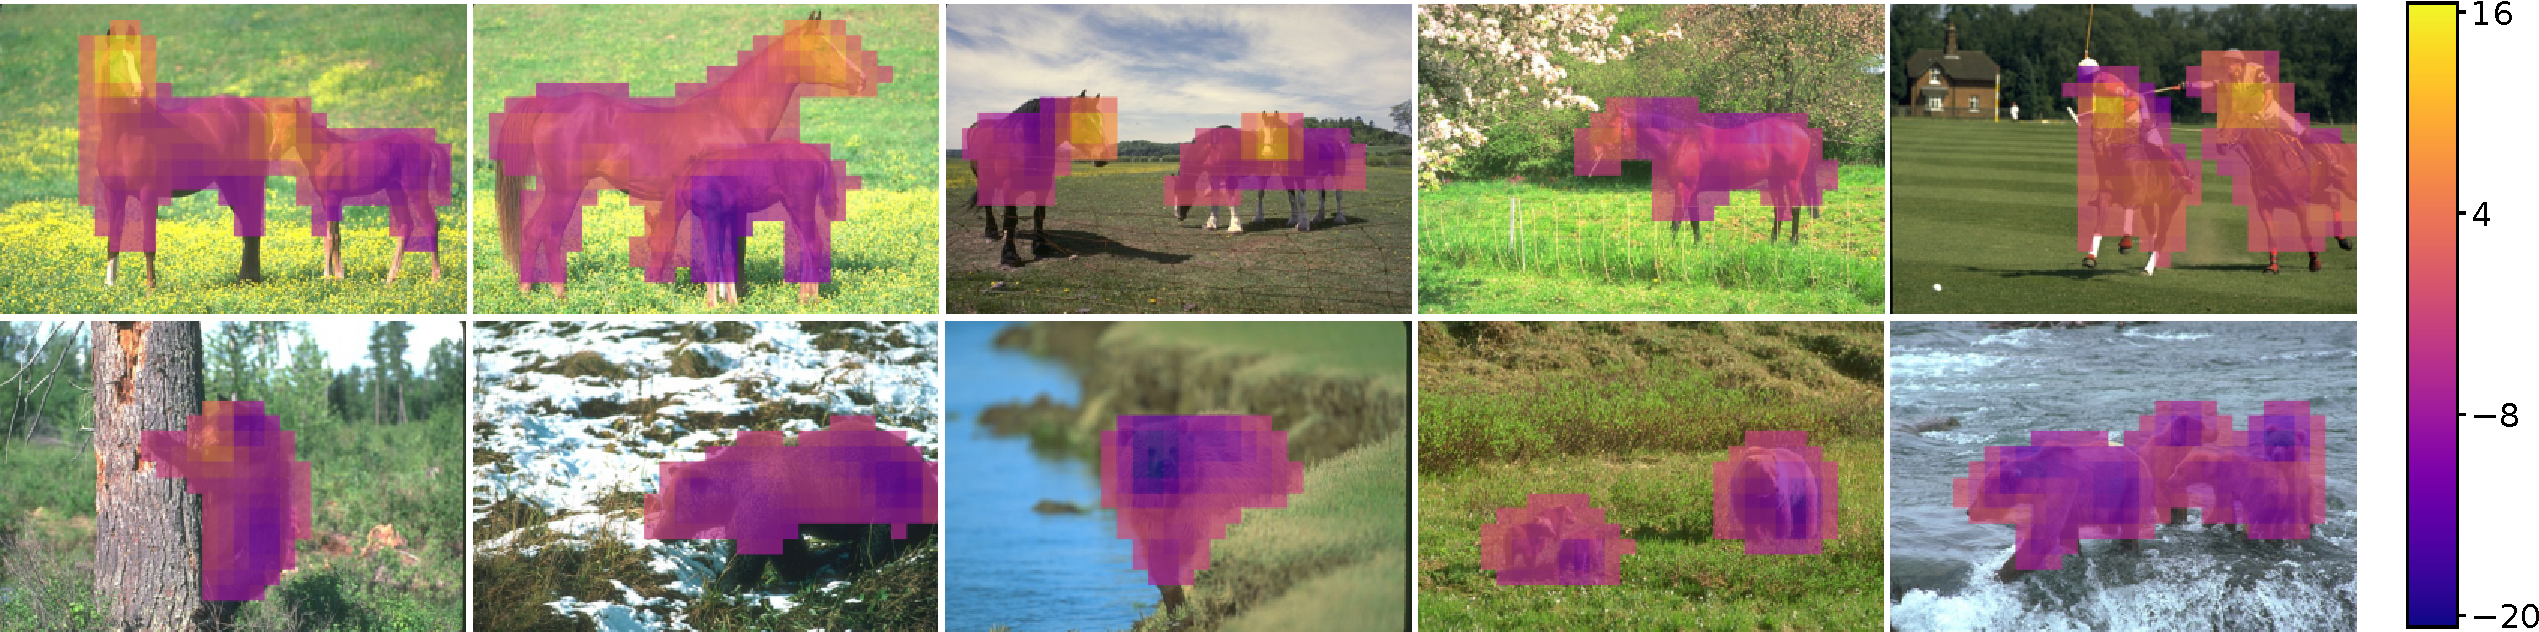
\includegraphics[width=\textwidth]{figures/overlayed_differentiator.pdf}
    \caption{The activations of feature map 130 show large values in the areas covering the horse's head.}
    \label{fig:overlayed_differentiator}
\end{figure}

\subsection{Feature-Centric Analysis}

In the previous subsection, the $\Sigma$- and $\Gamma$-scores were calculated to rank feature maps based on the similarity of their distributions. In this subsection, we analyze pairs of feature maps to report similar feature channels on an intra- and inter-class level.

\subsubsection{Intra-Class Comparison}

Comparing pairs of feature maps in one class of images can reveal redundant feature maps that capture similar semantic information. The $\bar{\Delta}$-score can be adopted to report pairs of similarly distributed feature maps in one class:
\begin{equation}
    \Phi_{k,l}(C) = \bar{\Delta}_{k,l} (C, C).
\end{equation}
A small $\Phi$-score reports pairs of similar feature maps in one class and vice versa.

\autoref{fig:heatmaps} (a, b) shows the heat maps of the intra-class $\Phi$-scores calculated for $C_{\text{horses}}$ and $C_{\text{bears}}$. The figure shows that there are pairs of similar feature channels (bright yellow blocks) and dissimilar channels (dark purple blocks).

\begin{figure}
    \centering
    \begin{subfigure}{0.3\textwidth}
        \centering
        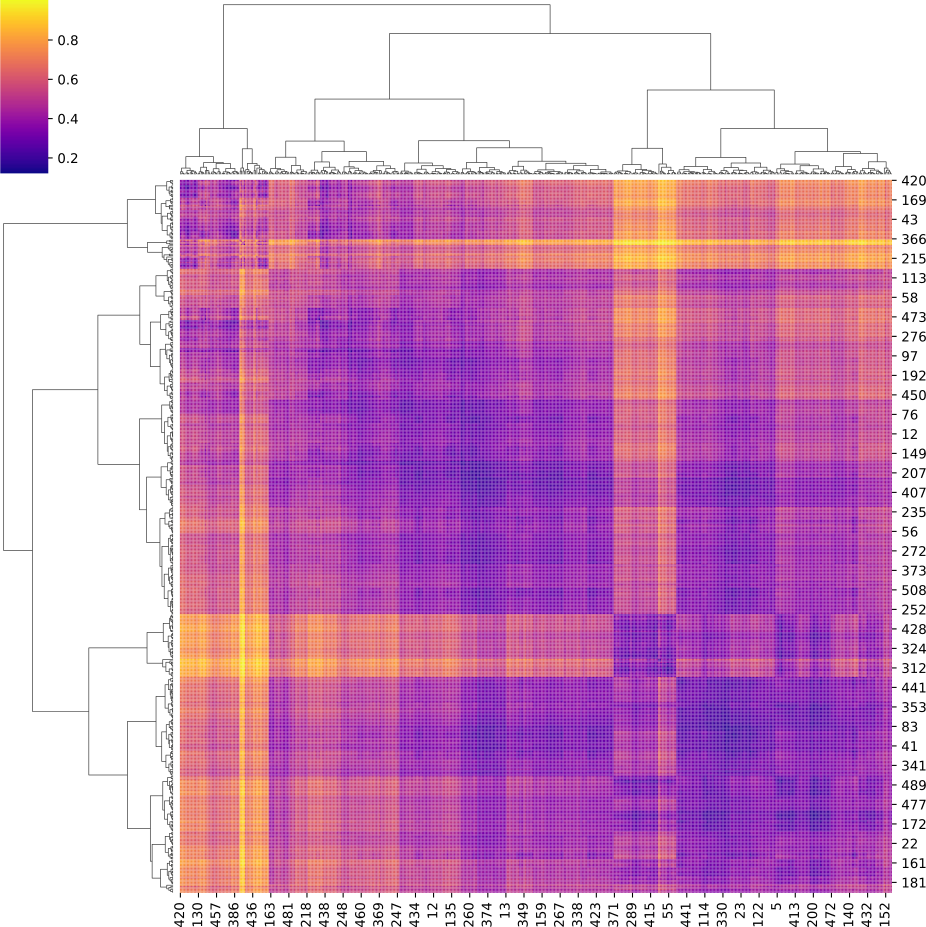
\includegraphics[width=\linewidth]{figures/horses_h_scores_ward_20210804-002107.png}
        \caption{$\Phi(C_{\text{horses}})$}
    \end{subfigure}
    \begin{subfigure}{0.3\textwidth}
        \centering
        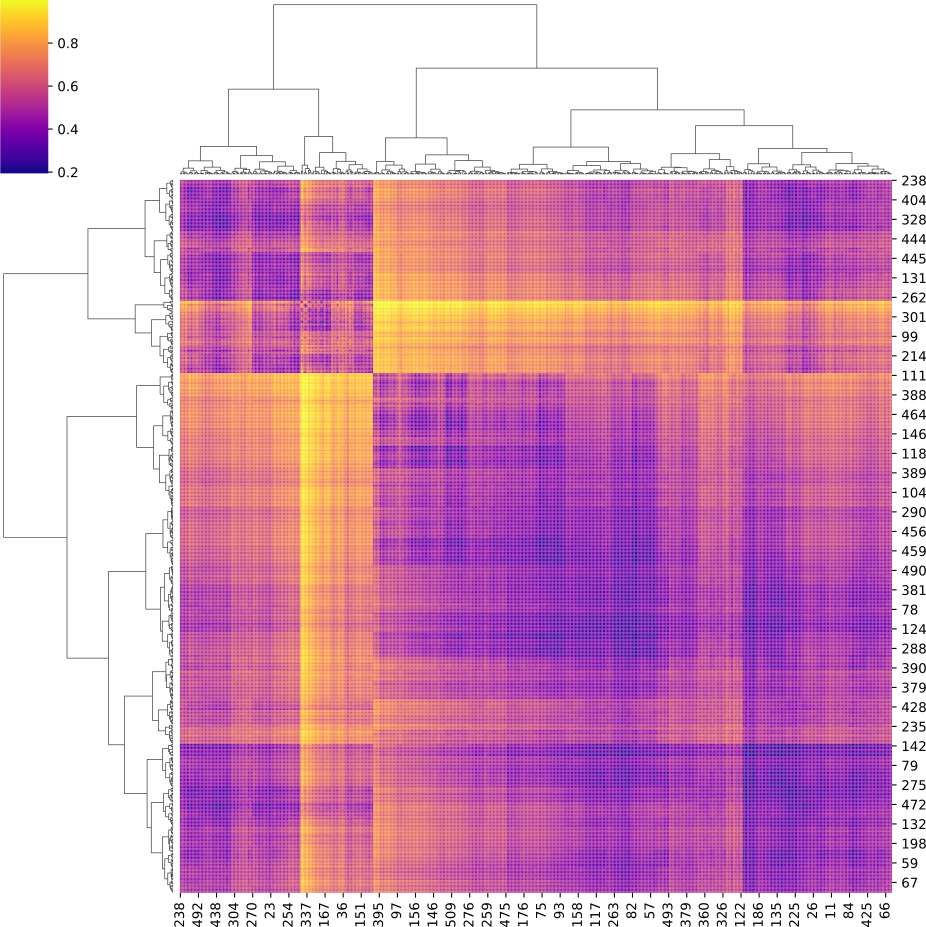
\includegraphics[width=\linewidth]{figures/bears_h_scores_ward_20210804-002107.png}
        \caption{$\Phi(C_{\text{bears}})$}
    \end{subfigure}
    \begin{subfigure}{0.3\textwidth}
        \centering
        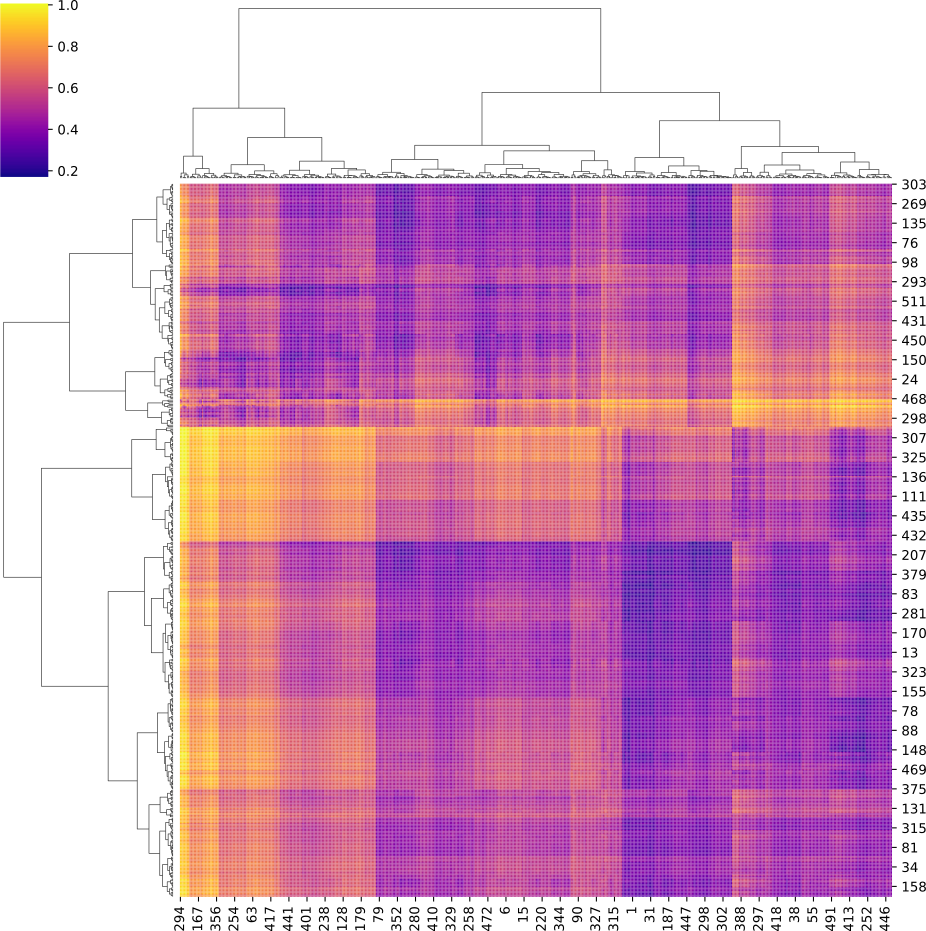
\includegraphics[width=\linewidth]{figures/combined_h_scores_ward_20210804-002107.png}
        \caption{$\bar{\Delta}(C_{\text{horses}}, C_{\text{bears}})$}
    \end{subfigure}
    \caption{Heat maps for comparing feature maps on an intra- (a,b) and inter-class (c) level.}
    \label{fig:heatmaps}
\end{figure}

\subsubsection{Inter-Class Comparison}

Analyzing pairs of feature maps from two classes of images can report the (dis-)similarly distributed feature maps, which can be used to show the similarities and differences between the two classes (according to the model). The $\bar{\Delta}$-scores (\autoref{eq:h_score}) can be used directly for this purpose.
As shown in \autoref{fig:heatmaps} (c), there are indeed blocks of similar colors. The dark purple (bright yellow) blocks represent feature maps that capture similarities (differences) found between the two classes.